         \chapter{Klassifikasie van Materie}\fancyfoot[LO,RE]{Chemie: Materie en Materiale}\label{chap:classification}
    \setcounter{figure}{1}
    \setcounter{subfigure}{1}
%     \label{09a7a4809656be0b739ee130746cd803}
%          \section{Mixtures, compounds and elements}
%     \nopagebreak
    \label{m38708*cid1}
            \section{Materiale}
            \nopagebreak
            \label{m38708} $ \hspace{-5pt}\begin{array}{cccccccccccc}   
\includegraphics[width=0.75cm]{col11305.imgs/summary_fullmarks.png} &   \end{array} $ \hspace{2 pt}\raisebox{-5 pt}{} {(section shortcode: P10011 )} \par 

            \label{m38708*id62175}Alles wat ons in die wêreld rondom ons sien is gemaak van materie. Die lug wat ons inasem, die grond waarop ons loop, die kos wat ons eet, die diere en plante wat rondom ons is, bestaan uit materie. Selfs ons eie menslike liggaam is gemaak van materie!\par 
            
            \begin{minipage}{.5\textwidth}
      \label{m38708*id62185}Verskillende voorwerpe kan van verskillende soorte \textbf{materiale} (stowwe) gemaak word (die materie waarvan voorwerpe gemaak word). Byvoorbeeld, 'n kas ('n \textsl{voorwerp}) word van hout, spykers, skarniere en knoppe (die \textsl{materiaal}) gemaak. Die \textbf{eienskappe} van die materiaal beïnvloed die eienskappe van die voorwerp. In die voorbeeld van die kas, maak die sterkte van die hout en metaal die kas sterk en duursaam. Elektriese drade word van metaal (bv. koper) gemaak omdat metale 'n tipe stof is wat kan elektrisiteit gelei. Dit is baie belangrik om die eienskappe van materiale of stowwe te verstaan sodat ons dit kan gebruik in ons huise, die industrie en op ander gebiede. In hierdie hoofstuk, sal ons kyk na verskillende soorte materiale en hulle eienskappe.\par 
\end{minipage}
\begin{minipage}{.5\textwidth}
\begin{center}
 \includegraphics[width=.8
\textwidth]{photos/cupboardby-grongar-flickr.jpg}\par
\textit{Prent verskaf deur grongar op Flickr.com}
\end{center}
\end{minipage} \\
\label{m38708*id0132}Sommige van die eienskappe van materie wat jy behoort te ken is:
\label{m38708*lid825}\begin{itemize}[noitemsep]
  \item Materiale (stowwe) kan \textbf{sterk} wees en weerstand bied teen buiging (bv. bakstene, rotse) of \textbf{swak} en maklik buigbaar (bv. klere).
  \item Materiale wat hitte gelei (bv. metale) word \textbf{termiese geleiers} genoem. Materiale wat elektrisiteit gelei (bv. koperdraad) is \textbf{elektriese geleiers}.
  \item \textbf{Bros} materiale breek maklik (bv. plastiek). Materiale wat \textbf{smeebaar} is (bv. klei, deeg), kan maklik in verskillende vorms gevorm word. Smeebare materiale kan in lang drade uitgerek word (bv. koper).
  \item \textbf{Magnetiese} materiale het 'n magnetiese veld (bv. yster).
  \item \textbf{Digtheid} is die massa per eenheid volume. By voorbeeld, klippe is digter as beton en beton is digter as modder.
  \item Die \textbf{kook- en smeltpunte} van stowwe vertel ons van die temperatuur waarteen die stof sal kook of smelt. Dit help ons om stowwe te klassifiseer as vastestowwe, vloeistowwe of gasse by 'n spesifieke temperatuur.\end{itemize}
\par 

      \label{m38708*id62556}Die diagram hieronder toon 'n manier waarvolgens materie geklassifiseer (gegroepeer) kan word volgens verskillende eienskappe. As jy verder lees in hierdie hoofstuk, sal jy sien dat daar ook ander maniere van die klassifikasie van stowwe is, byvoorbeeld of die stof 'n goeie elektriese geleier is of nie.\par 
    \setcounter{subfigure}{0}
	\begin{figure}[H] % horizontal\label{m38708*uid1}
    \begin{center}
\scalebox{.8}{
\begin{pspicture}(-6,0.5)(6,5)
%\psgrid[gridcolor=lightgray]
\rput(0,4.8){\textbf{MATERIE}}
\psline(-3,4)(-3,4.4)(3,4.4)(3,4)
\rput(-3,3.8){\textbf{MENGSELS}}
\rput(3,3.8){\textbf{SUIWER  STOWWE}}
\psline(-3,3.4)(-3,3.6)
\psline(3,3.4)(3,3.6)
\psline(-4.5,3)(-4.5,3.4)(-1.5,3.4)(-1.5,3)
\psline(4.5,3)(4.5,3.4)(1.5,3.4)(1.5,3)
\rput(-4.5,2.8){Homogene}
\rput(-1.5,2.8){Heterogene}
\rput(4.5,2.8){Verbindings}
\rput(1.5,2.8){Elemente}
\psline(1.5,2.6)(1.5,2.4)
\psline(0,2.0)(0,2.4)(3,2.4)(3,2.0)
\rput(0,1.8){Metale}
\rput(3,1.8){Nie-metale}
\psline(0,1.4)(0,1.6)
\psline(-1.5,1.2)(-1.5,1.4)(1.5,1.4)(1.5,1.2)
\rput(-1.5,1){Magneties}
\rput(1.5,1){Nie-magneties}
%\psset{yunit=0.5}
\end{pspicture}
}
    \end{center}
\caption{Klassifikasie van materie.}
\label{fig:c:ClassificationOfMatter}
 \end{figure} \vspace{-1cm}      
    \label{m38708*eip-344}\begin{activity}{Uit watter stowwe word produkte gemaak?}
{
\begin{minipage}{.5\textwidth}
Hierdie aktiwiteit let op die stowwe waaruit voedselprodukte saamgestel is. In groepe van 3 of 4 kyk na die etikette op kositems. Maak 'n lys van die bestanddele. Kan jy (deur na die bestanddele te kyk) s\^e watter kos dit is (d.w.s. speserye, olie, lekkers, ens.)? Voedselprodukte word gemerk om vir jou as verbruiker te help om te weet wat jy eet asook met die keuse van gesonder alternatiewe. Sommige kunsmatige smaakmiddels en kleurmiddels, soos mononatrium glutamaat (MSG van die Engels ``Monosodium Glutamate'') en tartrasien word deesdae minder in kosse gebruik vir gesondheidsredes. Is daar ander bestanddele in die produkte wat onveilig is om te eet? Watter preserveermiddels en byvoegings (bv. tartrasien, MSG, kleurmiddels) is daar? Is hierdie preserveermiddels en byvoegings goed vir jou? Is daar natuurlike (van plante afkomstig) alternatiewe? Wat gebruik verskillende inheemse groepe mense om hulle kos te geur en te bewaar?
\end{minipage}
\begin{minipage}{.5\textwidth}
 \begin{center}
 \includegraphics[width=.8\textwidth]{photos/food_labels.png}\par
\end{center}
\end{minipage}

 }  \end{activity}
\begin{activity}{Klassifiseer stowwe} {
\begin{minipage}{.4\textwidth}
Kyk rondom jou na verskillende strukture. Maak 'n lys van al die verskillende materiale wat jy sien. Probeer om uit te werk waarom 'n spesifieke materiaal gebruik is. Kan jy al die verskillende materiale wat gebruik is volgens hul eienskappe klassifiseer? Waarom is hierdie materiale bo ander materiale gekies?
\end{minipage}
\begin{minipage}{.3\textwidth}
\begin{center}
 \includegraphics[height=.7\textwidth]{photos/windmillby-flowcomm-flickr.jpg}\par
\textit{Prent verskaf deur flowcomm op Flickr.com}
\end{center}
\end{minipage}
\begin{minipage}{.3\textwidth}
\begin{center}
 \includegraphics[height=.7\textwidth]{photos/materials.png}\par
\end{center}
\end{minipage}
}
\end{activity}


\label{m38708*cid2}
            \section{Mengsels}
            \nopagebreak
            \label{m38708*id62584}Ons sien die hele tyd mengsels in ons alledaaglikse lewe. 'n Bredie is, byvoorbeeld, 'n mengsel van verskillende voedselsoorte soos vleis en groente, seewater is 'n mengsel van water, sout en ander stowwe, en die lug is 'n mengsel van gasse soos koolstofdioksied, suurstof en stikstof.\par 
\label{m38708*fhsst!!!underscore!!!id69}
\Definition{\label{id2405672}Mengsel} {\label{m38708*meaningfhsst!!!underscore!!!id69}
      'n Mengsel word uit twee of meer stowwe saamgestel. Hierdie stowwe is nie verbind of aanmekaar geheg nie en geen chemiese reaksie het plaasgevind nie.
       } 
      \label{m38708*id62612}Die stowwe waaruit die mengsel bestaan:\par 
      \label{m38708*id62615}\begin{itemize}[noitemsep]
            \label{m38708*uid2}\item \textbf{word nie in 'n vaste verhouding gemeng nie.} \\
Verbeel jou jy het 250 ml water en jy voeg sand by die water. Dit maak nie saak of jy 20 g, 40 g, 100 g of enige ander massa sand by die water voeg nie, dit sal steeds 'n mengsel van sand en water wees.
\label{m38708*uid3}\item \textbf{behou hul fisiese eienskappe.} \\
In die voorbeeld wat ons gebruik het, het nie een van die stowwe op enige manier verander toe hulle saam gemeng is nie. Die sand is nog sand en die water is nogsteeds water.
\label{m38708*uid4}\item \textbf{kan op 'n meganiese wyse geskei word.} \\
Om iets volgens ``meganiese wyse'' te skei, beteken dat daar geen chemiese proses betrokke was nie. In ons sand en water voorbeeld, is dit moontlik om die mengsel te skei deur eenvoudig die water deur 'n filter te giet. Iets \textsl{fisies} word met die mengsel gedoen, eerder as iets \textsl{chemies}.
\end{itemize}
      \label{m38708*id62700}Ons kan mengsels verder in twee hoofgroepe verdeel naamlik: heterogeen en homogeen.\par 

      \label{m38708*uid5}
            \subsection*{Heterogene Mengsels}
            \nopagebreak
        \label{m38708*id62715}'n \textbf{Heterogene} mengsel het nie' n definitiewe samestelling nie. Ontbytgraan in melk is 'n voorbeeld van' n heterogene mengsel. Grond is nog 'n voorbeeld. Grond het klippies, plantmateriaal en sand in. Alhoewel jy een stof by 'n ander stof voeg, bly hulle afsonderlik in die mengsel. Ons s\^e heterogene mengsels is \textsl{nie-uniform}, met ander woorde hulle is nie presies dieselfde regdeur nie.\par 
\begin{minipage}{.5\textwidth}
\begin{center}
 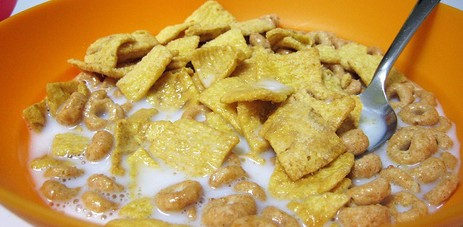
\includegraphics[width=.8\textwidth]{photos/mixtureby-dougww-flickr.jpg}\par
\textit{Prent verskaf deur dougww op Flickr.com}
\end{center}
\end{minipage}
\begin{minipage}{.5\textwidth}
\begin{figure}[H]
\label{fig:heterogeneousmixture}
\begin{center}
 \begin{pspicture}(0,-1)(11,4.7)
\SpecialCoor
\psframe[fillstyle=crosshatch*,fillcolor=white,hatchcolor=lightgray,hatchwidth=1.2pt,hatchsep=1.8pt,hatchangle=0](0,0)(4,4)
\pscircle[fillcolor=lightgray,fillstyle=solid](0.5,0.5){0.2}
\pscircle[fillcolor=white,fillstyle=solid](1,1.2){0.1}
\pscircle[fillcolor=lightgray,fillstyle=solid](2.1,1){0.2}
\pscircle[fillcolor=white,fillstyle=solid](2.3,0.4){0.1}
\pscircle[fillcolor=lightgray,fillstyle=solid](3.5,1){0.2}
\pscircle[fillcolor=white,fillstyle=solid](0.5,1.6){0.1}
\pscircle[fillcolor=white,fillstyle=solid](1,2){0.1}
\pscircle[fillcolor=white,fillstyle=solid](1.8,1.5){0.1}
\pscircle[fillcolor=lightgray,fillstyle=solid](2,2){0.2}
\pscircle[fillcolor=lightgray,fillstyle=solid](0.5,2.7){0.2}
\pscircle[fillcolor=lightgray,fillstyle=solid](2.3,2.5){0.2}
\pscircle[fillcolor=white,fillstyle=solid](2.5,2.8){0.1}
\pscircle[fillcolor=white,fillstyle=solid](3,3){0.1}
\pscircle[fillcolor=white,fillstyle=solid](3.5,2.4){0.1}
\pscircle[fillcolor=white,fillstyle=solid](0.5,3.5){0.1}
\pscircle[fillcolor=white,fillstyle=solid](2,3.4){0.1}
\pscircle[fillcolor=lightgray,fillstyle=solid](3.5,3.5){0.2}
\pscircle[fillcolor=lightgray,fillstyle=solid](1.7,3.1){0.2}
\pscircle[fillcolor=white,fillstyle=solid](3,3){0.1}
\end{pspicture}
\end{center}
\caption{'n Submikroskopiese voorstelling van 'n heterogene mengsel. Die grys sirkels stel een stof (bv. 'n ontbytgraan) en die wit sirkels is nog 'n stof (bv. 'n ander ontbytgraan) voor. Die agtergrond is die melk.}
\end{figure}
\end{minipage}


\label{m38708*fhsst!!!underscore!!!id89}\Definition{\label{id2405839} { Heterogene mengsel }} 
{ \label{m38708*meaningfhsst!!!underscore!!!id89}
        'n Heterogene mengsel is een wat bestaan uit twee of meer stowwe, is nie-uniform en die verskillende komponente van die mengsel kan gesien word.
         } 
Heterogene mengsels kan verder onderverdeel word na gelang daarvan of dit twee vloeistowwe is wat gemeng is, 'n vaste stof en 'n vloeistof of 'n vloeistof en 'n gas of selfs 'n gas en 'n vaste stof. Vir hierdie mengsels is spesiale name gegee soos jy in die tabel hieronder sien.   \par
\begin{table}[h!]
 \begin{center}
  \begin{tabular}{|l|l|l|}\hline
   \textbf{Fases van materie} & \textbf{Naam van mengsel} & \textbf{Voorbeeld} \\ \hline
   vloeistof-vloeistof & emulsie & olie en water \\ \hline
   vaste stof-vloeistof & suspensie & modderige \\ \hline
   gas-vloeistof & a\"erosol & bruisdrankies \\ \hline
   gas-vastestof & rook & rookmis \\ \hline
  \end{tabular}

 \end{center}
\caption{Voorbeelde van verskillende heterogene mengsels}
\label{tab:mixtures}
\end{table}

      \label{m38708*uid6}
            \subsection*{Homogene mengsels}
            \nopagebreak
        \label{m38708*id62762}'n \textbf{Homogene} mengsel het 'n definitiewe samestelling en spesifieke eienskappe. In 'n homogene mengsel kan die verskillende dele nie gesien word nie. 'n Oplossing van sout in water is 'n voorbeeld van 'n homogene mengsel. Wanneer die sout oplos, versprei dit eweredig deur die water sodat alle dele van die oplossing dieselfde is, jy kan nie meer die sout geskei van die water sien nie. Dink ook aan koffie sonder melk. Die lug wat ons inasem, is nog 'n voorbeeld van 'n homogene mengsel, want dit bestaan uit verskillende gasse wat in 'n konstante verhouding gemeng is, wat nie visueel van mekaar onderskei kan word nie (d.w.s. jy kan nie die verskillende komponente sien nie).\par 
\begin{minipage}{.5\textwidth}
\begin{center}
 \includegraphics[width=.3\textwidth]{photos/coffeeby_JuliusSchorzman_wikimedia.jpg}\par
\textit{Prent verskaf deur Julius Schorzman op wikimedia}
\end{center}
\end{minipage}
\begin{minipage}{.5\textwidth}
\begin{center}
 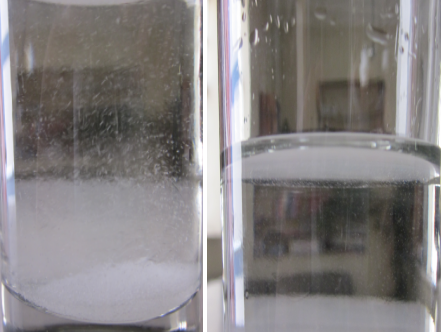
\includegraphics[width=.5\textwidth]{photos/saltwater.png}\par
\end{center}
\end{minipage}
\label{m38708*fhsst!!!underscore!!!id96}\Definition{   \label{id2405912}Homogene mengsel} { \label{m38708*meaningfhsst!!!underscore!!!id96}
        'n Homogene mengsel is een wat uniform (eenvormig) is, en waar die verskillende komponente van die mengsel nie gesien kan word nie.
         } 
%         \label{m38708*id62795}An \textbf{alloy} is a homogeneous mixture of two or more elements, at least one of which is a metal, where the resulting material has metallic properties. Alloys are usually made to improve the properties of the elements that make them up. For example steel is much stronger than iron (which is the main component of steel). Steel is a mixture (alloy) of mainly iron with carbon (to make it harder), manganese (to make it strong) and chromium (to prevent rusting).\par 
\vspace{-2cm}
\label{m38708*eip-479}
      \begin{wex}{Mengsels}
{Vir elk van die volgende mengsels s� of dit 'n homogene of 'n heterogene mengsel is:
\label{m38708*eip-id1167649056231}\begin{enumerate}[noitemsep, label=\textbf{\alph*}. ] 
            \leftskip=20pt\rightskip=\leftskip\item suiker opgelos in water
\item koekmeel en ystervylsels (klein stukkies yster)
\item koekmeel en bakpoeier
\item smarties, jellie tots en pepermente\end{enumerate} }
%  \par 
%\vspace{5pt}
%\label{m38708*eip-602}\noindent\textbf{Solution to Exercise }
%\label{m38708*eip-id7325184}
{\westep{Kyk na die definisie}
Ons kyk eers na die definisie van 'n heterogene en homogene mengsel.
\westep{Besluit of jy die komponente kan sien of nie.}
\begin{enumerate}[noitemsep, label=\textbf{\alph*}. ] 
 %           \leftskip=20pt\rightskip=\leftskip
\item Ons kan nie die suiker in die water sien nie.
\item Ons is in staat om stukkies yster in die koekmeel te sien.
\item Daar is geen manier om te onderskei tussen die koekmeel en bakpoeier nie.
\item Ons kan duidelik elk van die komponente waaruit die mengsel bestaan, sien. \end{enumerate}
\westep{Besluit of die komponente eenvormig gemeng is of nie}
\begin{enumerate}[noitemsep, label=\textbf{\alph*}. ] 
 %           \leftskip=20pt\rightskip=\leftskip
\item Die twee komponente is eenvormig gemeng.
\item In hierdie mengsel mag daar plekke wees daar baie ystervylsels is en plekke waar daar meer koekmeel is, dus is dit nie eenvormig gemeng nie.
\item Die twee komponente van die mengsel is eenvormig gemeng.
\item Die drie komponente van die mengsel is nie eweredig versprei nie.\end{enumerate}
\westep{Gee die finale antwoord
}
\begin{enumerate}[noitemsep, label=\textbf{\alph*}. ] 
 %           \leftskip=20pt\rightskip=\leftskip
\item Homogene mengsel.
\item Heterogene mengsel.
\item Homogene mengsel.
\item Heterogene mengsel.\end{enumerate}}
    \end{wex}
%    \end{mdframed}
 
 %   \noindent
\vspace{-1cm}
\begin{activity}{Die bereiding van mengsels}
{
\begin{minipage}{0.6\textwidth}
Maak mengsels van sand en water, kaliumdichromaat en water, jodium en etanol, jodium en water. Klassifiseer hierdie mengsels as heterogeen of homogeen. Gee redes vir jou keuse. Maak jou eie mengsels deur enige twee van die volgende bestanddele te gebruik \begin{itemize}[noitemsep] \item sand \item water \item klippe \item ontbytgraan \item sout \item suiker \end{itemize}Probeer om soveel verskillende mengsels as moontlik te maak. Klassifiseer elke mengsel en gee 'n rede vir jou antwoord.                                                                                                                                                                                                                                                                                                                                                                                                                       
\end{minipage}
\begin{minipage}{.4\textwidth}
{
\begin{center}
 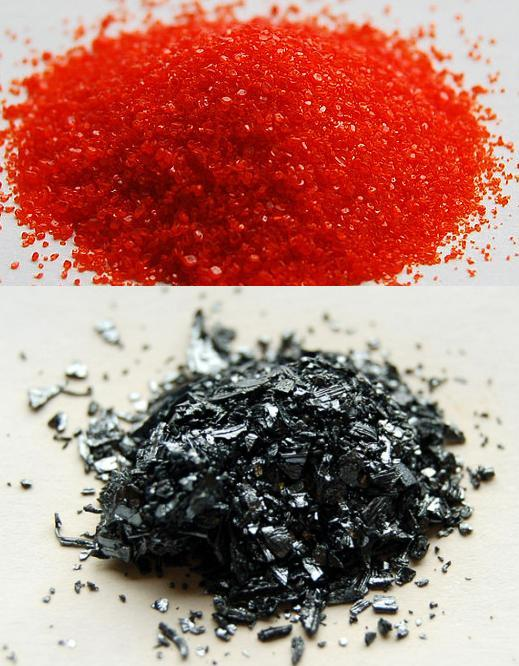
\includegraphics[width=.7\textwidth]{photos/iodine-KCr2O7-wikipedia.jpg}\par
\begin{caption}Kalium dichromaat (bo) and jodium (onder)\end{caption}
\end{center}
}

\end{minipage}
}
\end{activity}
\label{m38708*secfhsst!!!underscore!!!id169}
\begin{exercises}{Mengsels}
{Voltooi die volgende tabel: \par
%\nopagebreak
\begin{tabular}{|l|l|l|l|}\hline
\textbf{Stof} & \textbf{Nie-mengsel of} & \textbf{Heterogene} & \textbf{Homogene} \\ 
 & \textbf{mengsel} & \textbf{mengsel} & \textbf{mengsel} \\ \hline
kraanwater & & & \\ \hline
brons ('n allooi van koper en sink) & & & \\ \hline
beton & & & \\ \hline
aluminiumfolie & & & \\ \hline
Coca Cola & & & \\ \hline
seperige water & & & \\ \hline
swart tee & & & \\ \hline
suikerwater & & & \\ \hline
baba-melk formule & & & \\ \hline
\end{tabular}
    \label{m38708*cid3}
\par \raisebox{-5 pt}{
\includegraphics[width=0.5cm]{col11305.imgs/summary_www.png}} Vind die antwoorde met die kortkodes:
 \par \begin{tabular}[h]{cccccc}
 (1.) llm  & \end{tabular} }
\end{exercises}
            \section{Suiwer stowwe: Elemente en verbindings}
            \nopagebreak
      \label{m38708*id63273}Enige stof wat nie 'n mengsel is nie, word 'n \textbf{suiwer stof} genoem. Suiwer stowwe sluit \textbf{elemente} en \textbf{verbindings} in. Dit is baie moeiliker om suiwer stowwe in hul dele af te breek, ingewikkelde chemiese metodes is nodig om dit te doen. Chromatografie is die proses van die skeiding van stowwe in hul individuele komponente. As 'n stof suiwer is, sal chromatografie slegs 'n enkel stof aan die einde van die proses oplewer. As 'n stof onsuiwer is sal verskeie stowwe aan die einde van die proses sien.\par 
\begin{activity}{Voorgestelde praktiese aktiwiteit: Smartie chromatografie}{
Jy benodig:
\begin{itemize}[noitemsep]
\item filtreerpapier (of kladpapier)
\item 'n paar Smarties in verskillende kleure
\item water
\item an oogdrupper
\end{itemize}
\begin{minipage}{.5\textwidth}
Plaas 'n Smartie in die middel van 'n stukkie filtreerpapier. Drup versigtig 'n paar druppels water op die Smartie, totdat die Smartie goed nat is en daar 'n ring van water op die filtreerpapier vorm. Na 'n rukkie behoort jy 'n gekleurde ring op die papier rondom die Smartie waar te neem. Dit is omdat die voedselkleursel, wat gebruik was om die Smartie te kleur, in die water opgelos het en deur die papier weg van die Smartie af beweeg het.
\end{minipage}
\begin{minipage}{.5\textwidth}
\begin{center}
 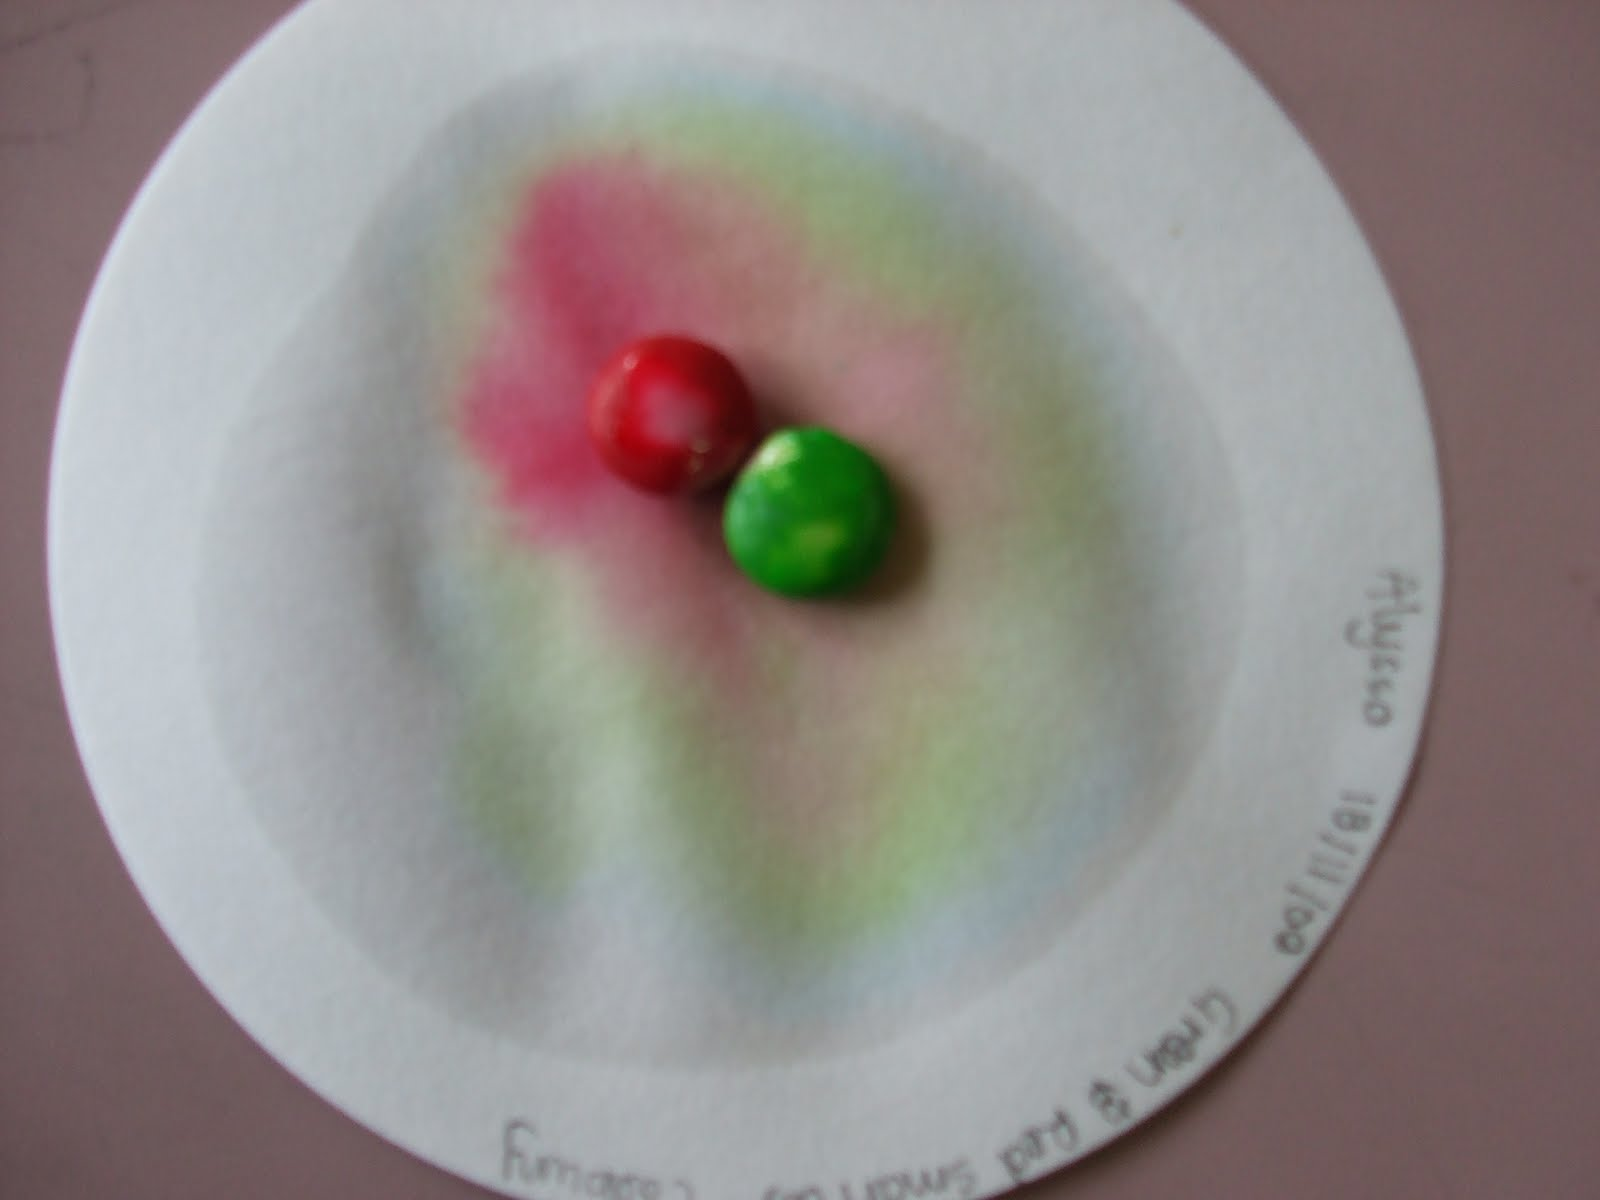
\includegraphics[width=.8\textwidth]{photos/smartie2.jpg}\par
\textit{Prent verskaf deur Neil Ravenscroft - UCT}
\end{center}
\end{minipage}
}
\end{activity}
\par 
	\par
      \label{m38708*uid25}
            \subsection*{Elemente}
            \nopagebreak
        \label{m38708*id63302}'n \textbf{Element} is 'n chemiese stof wat nie verdeel of verander kan word in ander chemiese stowwe deur gewone chemiese metodes nie. Die kleinste eenheid van 'n element is die \textbf{atoom}.\par 
\label{m38708*fhsst!!!underscore!!!id193}
\Definition{   \label{id2406278} Element } 
{ \label{m38708*meaningfhsst!!!underscore!!!id193}
'n Element is 'n stof wat nie in ander stowwe opgebreek kan word deur chemiese metodes nie.} 
        \label{m38708*id63334}Daar is amptelik 112 benoemde elemente waarvan omtrent 118 bekende elemente is. Meeste van hierdie elemente kom natuurlik voor, maar sommige is mensgemaak. Die elemente wat ons ken word in die \textbf{Periodieke Tabel van die Elemente} voorgestel. Elke element word tot 'n \textbf{chemiese simbool} afgekort. Tabel \ref{tab:elements} gee die eerste 20 elemente en 'n paar van die algemene oorgangsmetale.\par \label{m38708*eip-775}
\begin{table}[h!]
\label{tab:elements}
\begin{center}
\begin{tabular}{|l|l|l|l|}\hline
\textbf{Element naam} & \textbf{Element simbool} & \textbf{Element naam} & \textbf{Element simbool} \\ \hline
Waterstof & $\text{H}$ & Fosfor & $\text{P}$  \\ \hline
Helium & $\text{He}$ & Swawel & $\text{S}$ \\ \hline
Litium & $\text{Li}$ & Chloor & $\text{Cl}$ \\ \hline
Berillium & $\text{Be}$ & Argon & $\text{Ar}$ \\ \hline 
Boor & $\text{B}$ & Kalium & $\text{K}$ \\ \hline
Koolstof & $\text{C}$ & Kalsium & $\text{Ca}$ \\ \hline 
Stikstof & $\text{N}$ & Yster & $\text{Fe}$ \\ \hline
Suurstof & $\text{O}$ & Nikkel & $\text{Ni}$ \\ \hline 
Fluoor & $\text{F}$ & Koper & $\text{Cu}$ \\ \hline
Neon & $\text{Ne}$  & Sink & $\text{Zn}$ \\ \hline
Natrium & $\text{Na}$  & Silwer & $\text{Ag}$ \\ \hline
Magnesium & $\text{Mg}$  & Platinum & $\text{Pt}$ \\ \hline
Aluminium & $\text{Al}$ & Goud & $\text{Au}$ \\ \hline
Silicon & $\text{Si}$ & Kwik & $\text{Hg}$  \\ \hline
\end{tabular}
\end{center}
\caption{Lys van die eerste 20 elemente en 'n paar algemene oorgangsmetale}
\end{table}
\par \vspace{-.5cm}
%\begin{tabular}{cc}
%	\hspace*{-50pt}\raisebox{-8 mm}{\hspace{-0.2in}
\includegraphics[width=0.75in]{col11305.imgs/psfact2.png} } & 
%	\begin{minipage}{0.85\textwidth}
%	\begin{note}
      \IFact{Onlangs is ooreengekom dat twee bykomende elemente tot die amptelike lys van benoemde elemente gevoeg word. Dit is elemente nommer 114 en 116. Die voorgestelde naam vir element 114 is flerovium en vir element 116 is dit moskovium. Dit bring die totale aantal amptelik benoemde elemente tot 114.}
%	\end{note}
%	\end{minipage}
%	\end{tabular}
	\par \vspace{-.5cm}
      \label{m38708*uid26}
            \subsection*{Compounds}
            \nopagebreak
        \label{m38708*id63363}A \textbf{compound} is a chemical substance that forms when two or more different elements combine in a fixed ratio. Water ($\text{H}{}_{2}\text{O}$), for example, is a compound that is made up of two hydrogen atoms for every one oxygen atom. Sodium chloride ($\text{NaCl}$) is a compound made up of one sodium atom for every chlorine atom. An important characteristic of a compound is that it has a \textbf{chemical formula}, which describes the ratio in which the atoms of each element in the compound occur.\par 
\label{m38708*fhsst!!!underscore!!!id201}
%\begin{definition}
%	  \begin{tabular*}{15 cm}{m{15 mm}m{}}
%	\hspace*{-50pt}  
\includegraphics[width=0.5in]{col11305.imgs/psflag2.png}   & 
\Definition{\label{id2406453} Compound } { \label{m38708*meaningfhsst!!!underscore!!!id201}
        A substance made up of two or more different elements that are joined together in a fixed ratio.
         } 
%       \end{tabular*}
%       \end{definition}
        \label{m38708*id63410} Figure \ref{fig:classification:mixture and compound} might help you to understand the difference between the terms \textbf{element}, \textbf{mixture} and \textbf{compound}. Iron ($\text{Fe}$) and sulphur ($\text{S}$) are two elements. When they are added together, they form a \textsl{mixture} of iron and sulphur. The iron and sulphur are not joined together. However, if the mixture is heated, a new \textbf{compound} is formed, which is called iron sulphide ($\text{FeS}$). \par 
%     \setcounter{subfigure}{0}
 \begin{minipage}{.5\textwidth}
    \begin{center}
\scalebox{0.8}{
 \begin{pspicture}(0,-1)(11,4.7)
\SpecialCoor
%\psgrid[gridcolor=lightgray]
\def\fe{\pscircle[fillcolor=violet!20!gray!70!blue,fillstyle=solid](0,0){0.4}\rput(0,0){Fe}}
\def\s{\pscircle[fillcolor=yellow,fillstyle=solid](0,0){0.2}\rput(0,0){S}}
\def\fes{\fe \rput(0.6,0){\s}} 

\psframe(0,0)(4,4)
\rput(1.5,2){\s}
\rput{30}(3,1){\rput(1,1){\fe}\rput(1.5,2){\s}}
\rput{65}(1.55,1.33){\rput(1,1){\fe}\rput(1.5,2){\s}}
\rput{265}(2,3){\rput(-0.1,0.4){\fe}\rput(1.5,1.6){\s}}
\rput(2,0.6){\s}
\rput(1,1){\fe}
\rput(3,0.7){\fe}
\rput(2.4,2){\fe}
\rput(1.4,3.6){\s}
\psline(3.4,0.6)(4.2,0.6)
\uput[r](4.2,0.6){\parbox{1.5cm}{An atom of the element iron (Fe)}}

\psline(3.5,3.5)(4.2,3.5)
\uput[r](4.2,3.5){\parbox{1.5cm}{An atom of the element sulfur (S)}}
% \rput(2,-0.5){\parbox{4cm}{A mixture of iron and sulphur}}

% \rput(7,0){
% \psframe(0,0)(4,4)
% \rput(1,2){\fes}
% \rput(1,1){\fes}
% \rput(3,0.7){\fes}
% \rput(1,3.5){\fes}
% \rput(3,3.2){\fes}
% \rput(2.4,2){\fes}
% \rput(2,-0.5){\parbox{4cm}{The compound iron sulphide (FeS)}}}

\end{pspicture}
}\\
\begin{caption}A mixture of iron and sulphur\end{caption}
\label{fig:classification:mixture and compound}
    \end{center}
\end{minipage}
 \begin{minipage}{.5\textwidth}
  \begin{center}
   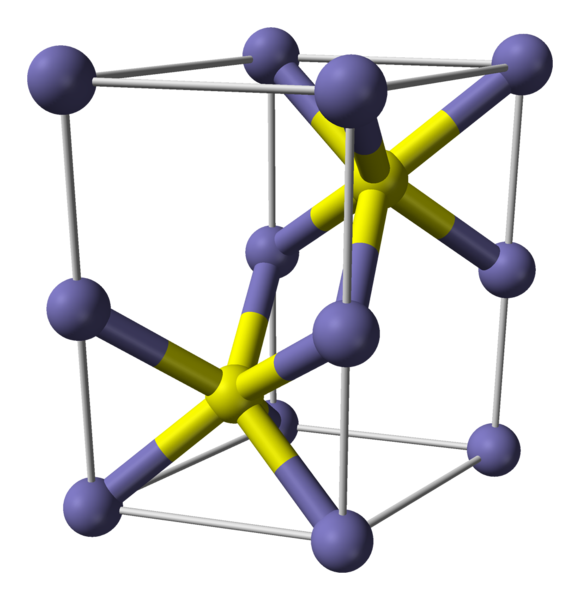
\includegraphics[width=0.4\textwidth]{photos/FeS_wikipedia.png}\\
\begin{caption}A model of the iron sulphide crystal\end{caption}
  \end{center}

 \end{minipage}

\label{m38708*eip-487} Figure \ref{fig:classification:mixture and compound} shows the submicroscopic representation of mixtures and compounds. In a submicroscopic representation we use circles to represent different elements. To show a compound, we draw several circles joined together. Mixtures are simply shown as two or more individual elements in the same box. The circles are not joined for a mixture.\par 
\label{m38708*id0124}We can also use symbols to represent elements, mixtures and compounds. The symbols for the elements are all found on the periodic table. Compounds are shown as two or more element names written right next to each other. Subscripts may be used to show that there is more than one atom of a particular element. (e.g. $\text{H}{}_{2}\text{O}$ or $\text{NH}_{3}$). Mixtures are written as: a mixture of element (or compound) A and element (or compound) B. (e.g. a mixture of $\text{Fe}$ and $\text{S}$).\par 
\label{m38708*eip-524}
      \begin{wex}
{Mixtures and pure substances}
{For each of the following substances state whether it is a pure substance or a mixture. If it is a mixture, is it homogenous or heterogenous? If it is a pure substance is it an element or a compound? 
\label{m38708*eip-id1167351497334}\begin{enumerate}[noitemsep, label=\textbf{\alph*}. ] 
   %         \leftskip=20pt\rightskip=\leftskip
\item Blood (which is made up from plasma and cells)
\item Argon
\item Silicon dioxide (${\text{SiO}}_{2}$)
\item Sand and stones
\end{enumerate}
  }
%\vspace{5pt}
%\label{m38708*eip-62}\noindent\textbf{Solution to Exercise }
%\label{m38708*eip-id1167366034146}
{
\westep{Apply the definitions}
An element is found on the periodic table, so we look at the periodic table and find that only argon appears there. Next we decide which are compounds and which are mixtures. Compounds consist of two or more elements joined in a fixed ratio. Sand and stones are not elements, neither is blood. But silicon is, as is oxygen. Finally we decide whether the mixtures are homogeneous or heterogeneous. Since we cannot see the seperate components of blood it is homogeneous. Sand and stones are heterogeneous.
 %           \leftskip=20pt\rightskip=\leftskip
\westep{Write the answer}
\begin{enumerate}
[noitemsep, label=\textbf{\alph*}. ]
\item Blood is a homogeneous mixture.
\item Argon is a pure substance. Argon is an element.
\item Silicon dioxide is a pure substance. It is a compound.
\item Sand and stones form a heterogeneous mixture.
\end{enumerate}}
    \end{wex}
%    \end{mdframed}
%    }
%    \noindent
\vspace{-1cm}
  \label{m38708*eip-326}
\begin{activity}{Using models to represent substances}{
\begin{minipage}{.5\textwidth}
The following substances are given:
\label{m38708*eip-id1166921187210}
\begin{itemize}[noitemsep]
    \item Air (consists of oxygen, nitrogen, hydrogen, water vapour)
    \item Hydrogen gas ($\text{H}_2$)
    \item Neon gas
    \item Steam
    \item Ammonia gas ($\text{NH}_3$)
\end{itemize}
\noindent
\begin{enumerate}[noitemsep, label=\textbf{\arabic*}.]
\item Use coloured balls to build models for each of the substances given.
\item Classify the substances according to elements, compounds, homogeneous mixtures, heterogeneous mixture, pure substance, impure substance.
\item Draw submicroscopic representations for each of the above examples.
\end{enumerate}
\end{minipage}
\begin{minipage}{.5\textwidth}
\begin{center}
 \includegraphics[width=.8\textwidth]{photos/models_classification.jpg}\par
\end{center}
\end{minipage}
}
\end{activity}
%NTS add image here 
\par \label{m38708*secfhsst!!!underscore!!!id212}
            \begin{exercises}{Elements, mixtures and compounds}{
            \nopagebreak
            \label{m38708*id63472}
 \begin{enumerate}[noitemsep, label=\textbf{\arabic*}. ] 
            \label{m38708*uid28}
    \item In the following table, tick whether each of the substances listed is a \textsl{mixture} or a \textsl{pure substance}. If it is a mixture, also say whether it is a homogeneous or heterogeneous mixture.
    % \textbf{m38708*id63499}\par
          \begin{table}[H]
    % \begin{table}[H]
    % \\ 'id2876023' '1'
        \begin{center}
      \label{m38708*id63499}
    \noindent
      \begin{tabular}{|l|l|l|}\hline
        \textbf{Substance} &
        \textbf{Mixture or pure} &
        \textbf{Homogeneous or heterogeneous mixture} \\ \hline
        fizzy colddrink & & \\ \hline
        steel & & \\ \hline
        oxygen & & \\ \hline
        iron filings & & \\ \hline
        smoke & & \\ \hline
        limestone (${\text{CaCO}}_{3}$) & & \\ \hline
    \end{tabular}
      \end{center}
%    \begin{center}{\small\bfseries Table 1.1}\end{center}
%    \begin{caption}{\small\bfseries Table 1.1}\end{caption}
\end{table}
    \par
\label{m38708*uid29}\item In each of the following cases, say whether the substance is an element, a mixture or a compound.
\label{m38708*id63912}\begin{enumerate}[noitemsep, label=\textbf{\alph*}. ] 
            \label{m38708*uid30}\item $\text{Cu}$
\label{m38708*uid31}\item iron and sulphur
\label{m38708*uid32}\item $\text{Al}$
\label{m38708*uid33}\item $\text{H}{}_{2}\text{SO}{}_{4}$\label{m38708*uid34}\item $\text{SO}{}_{3}$\end{enumerate}
                \end{enumerate}
    \label{m38708*cid4}
\par \raisebox{-5 pt}{
\includegraphics[width=0.5cm]{col11305.imgs/summary_www.png}} Find the answers with the shortcodes:
 \par \begin{tabular}[h]{cccccc}
 (1.) lly  &  (2.) llV  & \end{tabular}}
\end{exercises}
%NTS DIAGRAM is needed here and some more examples in the above exercises
            \section{Giving names and formulae to substances}
            \nopagebreak
      \label{m38708*eip-379}Think about what you call your friends. Some of your friends might have full names (long names) and a nickname (short name). These are the words we use to tell others who or what we are referring to. Their full name is like the substances name and their nickname is like the substances formulae. Without these names your friends would have no idea which of them you are referring to. Chemical substances have names, just like people have names. This helps scientists to communicate efficiently.     \par \label{m38708*id64028}It is easy to describe elements and mixtures. We simply use the names that we find on the periodic table for elements and we use words to describe mixtures. But how are compounds named? In the example of iron sulphide that was used earlier, the compound name is a combination of the names of the elements but slightly changed. \par 
      \label{m38708*id64033}The following are some guidelines for naming compounds:\par 
      \label{m38708*id64037}\begin{enumerate}[noitemsep, label=\textbf{\arabic*}. ] 
            \label{m38708*uid35}\item The compound name will always include the \textbf{names of the elements} that are part of it.
\label{m38708*id64059}\begin{itemize}[noitemsep]
            \label{m38708*uid36}\item A compound of \textbf{iron} ($\text{Fe}$) and \textsl{sulphur} ($\text{S}$) is \textbf{iron}\hspace{1ex}\textsl{sulph}ide ($\text{FeS}$)
\label{m38708*uid37}\item A compound of \textbf{potassium} ($\text{K}$) and \textsl{bromine} ($\text{Br}$) is \textbf{potassium}\hspace{1ex}\textsl{brom}ide ($\text{KBr}$)
\label{m38708*uid38}\item A compound of \textbf{sodium} ($\text{Na}$) and \textsl{chlorine} ($\text{Cl}$) is \textbf{sodium}\hspace{1ex}\textsl{chlor}ide ($\text{NaCl}$)
\end{itemize}
        \label{m38708*uid39}\item In a compound, the element that is on the left of the Periodic Table, is used \textsl{first} when naming the compound. In the example of $\text{NaCl}$, sodium is a group 1 element on the left hand side of the table, while chlorine is in group 7 on the right of the table. Sodium therefore comes first in the compound name. The same is true for $\text{FeS}$ and $\text{KBr}$.
\label{m38708*uid40}\item The \textbf{symbols} of the elements can be used to represent compounds e.g. $\text{FeS}$, $\text{NaCl}$, $\text{KBr}$ and $\text{H}{}_{2}\text{O}$. These are called \textbf{chemical formulae}. In the first three examples, the ratio of the elements in each compound is 1:1. So, for $\text{FeS}$, there is one atom of iron for every atom of sulphur in the compound. In the last example ($\text{H}{}_{2}\text{O}$) there are two atoms of hydrogen for every atom of oxygen in the compound.
\item A compound may contain \textbf{ions} (an ion is an atom that has lost or gained electrons). These ions can be either simple (consist of only one element) or compound (consist of several elements). Some of the more common ions and their formulae are given in table \ref{tab:cations} and in table \ref{tab:anions}. You should know all these ions.\\

    % \textbf{m38708*id64235}\par
    %      \begin{table}[H]
    % \begin{table}[H]
    % \\ 'id2876536' '1'
      
\begin{table}[H]
\begin{center}
\label{tab:cations}
\begin{tabular}{|l|c|l|c|l|c|l|c|} \hline
\textbf{Compound ion} & \textbf{Formula} & \textbf{Compound ion} & \textbf{Formula} & \textbf{Compound ion} & \textbf{Formula}  \\ \hline
Hydrogen       & $\text{H}^{+}$   & Lithium        & $\text{Li}^{+}$     & Sodium          & $\text{Na}^{+}$  \\ \hline
Potassium      & $\text{K}^{+}$   & Silver         & $\text{Ag}^{+}$     & Mercury (I)     & $\text{Hg}^{+}$  \\ \hline
Copper (I)     & $\text{Cu}^{+}$  & Ammonium       & $\text{NH}_{4}^{+}$ & Beryllium       & $\text{Be}^{2+}$ \\ \hline
Magnesium      & $\text{Mg}^{2+}$ & Calcium        & $\text{Ca}^{2+}$    & Barium          & $\text{Ba}^{2+}$ \\ \hline
Tin (II)       & $\text{Sn}^{2+}$ & Lead (II)      & $\text{Pb}^{2+}$    & Chromium (II)   & $\text{Cr}^{2+}$ \\ \hline
Manganese (II) & $\text{Mn}^{2+}$ & Iron (II)      & $\text{Fe}^{2+}$    & Cobalt (II)     & $\text{Co}^{2+}$ \\ \hline
Nickel         & $\text{Ni}^{2+}$ & Copper (II)    & $\text{Cu}^{2+}$    & Zinc            & $\text{Zn}^{2+}$ \\ \hline
Aluminium      & $\text{Al}^{3+}$ & Chromium (III) & $\text{Cr}^{3+}$    & Iron (III)      & $\text{Fe}^{3+}$ \\ \hline
Cobalt (III)   & $\text{Co}^{3+}$  & Chromium (VI)  & $\text{Cr}^{6+}$    & Manganese (VII) & $\text{Mn}^{7+}$ \\ \hline

\end{tabular}

 \end{center}
\caption{Table of cations}
\label{tab:cations}
\end{table}

\begin{table}[H]
\begin{center}
\label{tab:anions}
\begin{tabular}{|l|c|l|c|l|c|l|c|} \hline
\textbf{Compound ion} & \textbf{Formula}            & \textbf{Compound ion} & \textbf{Formula} \\ \hline
Fluoride             & $\text{F}^{-}$             & Oxide              & $\text{O}^{2-}$ \\ \hline
Chloride             & $\text{Cl}^{-}$            & Peroxide           & $\text{O}_{2}^{2-}$ \\ \hline
Bromide              & $\text{Br}^{-}$            & Carbonate          & $\text{CO}_{3}^{2-}$ \\ \hline
Iodide               & $\text{I}^{-}$             & Sulphide           & $\text{S}^{2-}$ \\ \hline
Hydroxide            & $\text{OH}^{-}$            & Sulphite           & $\text{SO}_{3}^{2-}$ \\ \hline
Nitrite              & $\text{NO}_{2}^{-}$        & Sulphate           & $\text{SO}_{4}^{2-}$ \\ \hline
Nitrate              & $\text{NO}_{3}^{-}$        & Thiosulphate       & $\text{S}_{2}{\text{O}}_{3}^{2-}$ \\ \hline
Hydrogen carbonate   & $\text{HCO}_{3}^{-}$       & Chromate           & $\text{CrO}_{4}^{2-}$ \\ \hline
Hydrogen sulphite    & $\text{HSO}_{3}^{-}$       & Dichromate         & $\text{Cr}_{2}{\text{O}}_{7}^{2-}$ \\ \hline
Hydrogen carbonate   & $\text{HSO}_{4}^{-}$       & Manganate          & $\text{MnO}_{4}^{2-}$ \\ \hline
Dihydrogen phosphate & $\text{H}_{2}{\text{PO}}_{4}^{-}$ & Oxalate   & $\text{(COO)}_{2}^{2-}/{\text{C}}_{2}{\text{O}}_{4}^{2-}$ \\ \hline
Hypochlorite         & $\text{ClO}^{-}$           & Hydrogen phosphate & $\text{HPO}_{4}^{2-}$ \\ \hline
Chlorate             & $\text{ClO}_{3}^{-}$       & Nitride            & $\text{N}^{3-}$ \\ \hline
Permanganate         & $\text{MnO}_{4}^{-}$       & Phosphate          & $\text{PO}_{4}^{3-}$ \\ \hline
Acetate Ethanoate    & $\text{CH}_{3}{\text{COO}}^{-}$   & Phosphide          & $\text{P}^{3-}$ \\ \hline
\end{tabular}

 \end{center}
\caption{Table of anions}
\label{tab:anions}
\end{table}

    \par
  \label{m38708*uid42}\item When there are only two elements in the compound, the compound is often given a \textbf{suffix} (ending) of -ide. You would have seen this in some of the examples we have used so far. For compound ions, when a non-metal is combined with oxygen to form a negative ion (anion) which then combines with a positive ion (cation) from hydrogen or a metal, then the suffix of the name will be ...ate or ...ite. $\text{NO}_{3}^{-}$ for example, is a negative ion, which may combine with a cation such as hydrogen ($\text{HNO}{}_{3}$) or a metal like potassium (KNO$_\text{3}$). The $\text{NO}_{3}^{-}$ anion has the name nitr\textbf{ate}. $\text{SO}_{3}^{2-}$ in a formula is sulph\textbf{ite}, e.g. sodium sulphite ($\text{Na}{}_{2}\text{SO}{}_{3}$).\newline
     $\text{SO}_{4}^{2-}$ is sulph\textbf{ate} and $\text{PO}_{4}^{3-}$ is phosph\textbf{ate}.
\label{m38708*uid43}\item \textbf{Prefixes} can be used to describe the ratio of the elements that are in the compound. This is used for non-metals. For metals, we add a roman number (I, II, III, IV) in brackets after the metal ion to indicate the ratio. You should know the following prefixes: 'mono' (one), 'di' (two) and 'tri' (three).
\label{m38708*id64977}\begin{itemize}[noitemsep]
            \label{m38708*uid44}\item $\text{CO}$ (carbon \textbf{mon}oxide) - There is one atom of oxygen for every one atom of carbon
\label{m38708*uid45}\item $\text{NO}{}_{2}$ (nitrogen \textbf{di}oxide) - There are two atoms of oxygen for every one atom of nitrogen
\label{m38708*uid46}\item $\text{SO}{}_{3}$ (sulphur \textbf{tri}oxide) - There are three atoms of oxygen for every one atom of sulphur
\end{itemize}
        \end{enumerate}
\label{m38708*id537402}The above guidelines also help us to work out the formula of a compound from the name of the compound.\par 
\label{m38708*eip-178}When working out the formula of a compound from the name we work backwards. For example, if you are given potassium chloride and were told to give its formula you would start by noting that we having potassium and chloride. Next you write down the formula for each of these ions. Potassium is ${\text{K}}^{+}$ and chloride is ${\text{Cl}}^{-}$. The final step is to note the charge on each ion to see how it combines. Since both potassium and chlorine have a charge of 1, they combine in a 1:1 ratio. The formula is $\text{KCl}$.\par \label{m38708*notfhsst!!!underscore!!!id252}
%\begin{tabular}{cc}
%	   \hspace*{-50pt}\raisebox{-8 mm}{ 
\includegraphics[width=0.5in]{col11305.imgs/pstip2.png}  }& 
%	\begin{minipage}{0.85\textwidth}
%	\begin{note}
      \Tip{
      \label{m38708*id65053}When numbers are written as 'subscripts' in compounds (i.e. they are written below and to the right of the element symbol), this tells us how many atoms of that element there are in relation to other elements in the compound. For example in nitrogen dioxide (${\text{NO}}_{2}$) there are two oxygen atoms for every one atom of nitrogen. Later, when we start looking at chemical equations, you will notice that sometimes there are numbers \textsl{before} the compound name. For example, $2\text{H}{}_{2}\text{O}$ means that there are two molecules of water, and that in each molecule there are two hydrogen atoms for every one oxygen atom. \par}  
%	\end{note}
%	\end{minipage}
%	\end{tabular}
	\par
\label{m38708*eip-163}We can use these rules to help us name both ionic compounds and covalent compounds. However, covalent compounds are often given other names by scientists to simplify the name (or because the molecule was named long before its formula was discovered). For example, if we have 2 hydrogen atoms and one oxygen atom the above naming rules would tell us that the substance is dihydrogen monoxide. But this compound is better known as water!  \par \label{m38708*eip-254} \vspace{-1cm} 
%      \noindent
%      \hspace*{-30pt}
\includegraphics[width=0.5in]{col11305.imgs/pspencil2.png}   \raisebox{25mm}{   
%      \begin{mdframed}[linewidth=4, leftmargin=40, rightmargin=40]  
      \begin{wex}{Writing chemical formulae 1}
{What is formula of sodium fluoride? 
\vspace{5pt}}
{\westep {List the ions involved:}
We have the sodium ion ($\text{Na}^{+}$) and the fluoride ion ($\text{F}^{-}$). (You can look these up on the tables of cations and anions.)
\westep{Write down the charges on the ions}
The sodium ion has a charge of $+1$ and the fluoride ion has a charge of $-1$.
\westep{Find the right combination}
For every plus, we must have a minus. So the $+1$ from sodium cancels out the $-1$ from fluoride. They combine in a $1:1$ ratio.
\westep{Write the formula}
$\text{NaF}$
}
\end{wex} \vspace{-2.5cm}
\begin{wex}{Writing chemical formulae 2}
{What is the formula for magnesium chloride?}
{\westep{List the ions involved}
$\text{Mg}^{2+}$ and $\text{Cl}^{-}$
\westep{Find the right combination}
Magnesium has a charge of $+2$ and would need two chlorides to balance the charge. They will combine in a 1:2 ratio. There is an easy way to find this ratio:
\begin{figure}[H] % horizontal\label{m38708*uid27}
    \begin{center}
 \begin{pspicture}(0,0)(2,2)
\SpecialCoor
\psline[linewidth=0.04]{->}(0,1)(1,0)
\uput[r](-1.2,1){\large{$\text{Mg}^{2+}$}}
\psline[linewidth=0.04]{->}(0,0)(1,1)
\uput[r](-1,0){\large{$\text{Cl}^{-}$}}
\uput[r](1,1){\large{$2$}}
\uput[r](1,0){\large{$1$}}

\end{pspicture}
\end{center}
\end{figure}
Draw a cross as above, and then you can see that $\text{Mg} \rightarrow 1$ and $\text{Cl} \rightarrow 2$. 
\westep{Write down the formula} 
$\text{MgCl}_2$
}
%\end{enumerate}}
    \end{wex}
%    \end{mdframed}
    
    \noindent
  \vspace{-3.5cm} 
      \noindent
      \begin{wex}{Writing chemical formulae 3}
{\label{m38708*eip-196}
  \label{m38708*eip-535}Write the chemical formula for magnesium oxide.
\vspace{5pt}
}
{
\westep{List the ions involved.}
$\text{Mg}^{2+}$ and $\text{O}^{2-}$
\westep{Find the right combination}
$\text{Mg}^{2+} : 2$ \newline
$\text{O}^{2-} : 2$ \newline
If you use the cross method, you will get a ratio of $2:2$. This ratio must always be in simplest form, i.e. $1:1$.
\westep{Write down the formula}
$\text{MgO}$ (\textboldface{not} $\text{Mg}_{2}\text{O}_{2}$) 
}
\end{wex} \vspace{-2.5cm}
\begin{wex}{Writing chemical formulae 4}
{Write the formula for copper(II) nitrate.}
{
\westep{List the ions involved}
$\text{Cu}^{2+}$ (the questions asks for copper(II) not copper(I)) \newline
$\text{NO}_{3}^{-}$
\westep{Find the right combination}
	\begin{figure}[H] % horizontal\label{m38708*uid27}
    \begin{center}
 \begin{pspicture}(0,0)(2,2)
\SpecialCoor
\psline[linewidth=0.04]{->}(0,1)(1,0)
\uput[r](-1,1){\large{$\text{Cu}^{2+}$}}
\psline[linewidth=0.04]{->}(0,0)(1,1)
\uput[r](-1.2,0){\large{$\text{NO}_{3}^{-}$}}
\uput[r](1,1){\large{$2$}}
\uput[r](1,0){\large{$1$}}

\end{pspicture}
\end{center}
\end{figure}
\westep{Write the formula}
${\text{Cu}}({\text{NO}}_{3})_{2}$
}
    \end{wex} \vspace{-2cm}
\Tip{Notice how in the last example we wrote $\text{NO}_{3}^{−}$ inside brackets. We do this to indicate that $\text{NO}_{3}^{−}$ is a compound ion and that there are two of these ions bonded to one copper ion.}
\begin{activity}{The ions dating game}
Your teacher will assign each of you a different ion (written on a piece of card). Stick this to yourself. You will also get cards with the numbers 1 - 5 on them. Now walk around the class and try to work out who you can pair up with and in what ratio. Once you have found a partner, indicate your ratio using the numbered cards. Check your results with your classmates or your teacher.
\end{activity}

  \label{m38708*secfhsst!!!underscore!!!id255}
            \begin{exercises}{Naming compounds}
{            \nopagebreak \noindent
      \label{m38708*id65118}\begin{enumerate}[noitemsep, label=\textbf{\arabic*}. ] 
            \label{m38708*uid47}\item The formula for calcium carbonate is $\text{CaCO}{}_{3}$.
\label{m38708*id65148}\begin{enumerate}[noitemsep, label=\textbf{\alph*}. ] 
            \label{m38708*uid48}\item Is calcium carbonate an element or a compound? Give a reason for your answer.
\label{m38708*uid49}\item What is the ratio of $\text{Ca}:\text{C}:\text{O}$ atoms in the formula?
\end{enumerate}
\label{m38708*uid50}\item Give the name of each of the following substances.
\label{m38708*id65189}\begin{enumerate}[noitemsep, label=\textbf{\alph*}. ] 
            \label{m38708*uid51}\item $\text{KBr}$
\label{m38708*uid52}\item $\text{HCl}$
\label{m38708*uid53}\item ${\text{KMnO}}_{4}$\label{m38708*uid54}\item ${\text{NO}}_{2}$\label{m38708*uid55}\item ${\text{NH}}_{4}\text{OH}$
\label{m38708*uid56}\item ${\text{Na}}_{2}{\text{SO}}_{4}$
\item ${\text{Fe}}({\text{NO}}_{3})_3$
\item ${\text{Pb}}{\text{SO}}_{3}$
\item ${\text{Cu}}({\text{HCO}}_{3})_2$
\end{enumerate}
\label{m38708*uid57}\item Give the chemical formula for each of the following compounds.
\label{m38708*id65338}\begin{enumerate}[noitemsep, label=\textbf{\alph*}. ] 
            \label{m38708*uid58}\item potassium nitrate
\label{m38708*uid59}\item sodium oxide
\label{m38708*uid60}\item barium sulphate
\label{m38708*uid61}\item aluminium chloride
\label{m38708*uid62}\item magnesium phosphate
\item tin(II) bromide
\item manganese(II) phosphide
\end{enumerate}
\end{enumerate}
    \label{m38708*cid5}
\par \raisebox{-5 pt}{
\includegraphics[width=0.5cm]{col11305.imgs/summary_www.png}} Find the answers with the shortcodes:
 \par \begin{tabular}[h]{cccccc}
 (1.) llp  &  (2.) lld  &  (3.) llv   & & \end{tabular}}
\end{exercises}
%The above exercise needs more examples and some diagrams! Possibly also lost a curly brace
            \section{Metals, Metalloids and Non-metals}
%ADD a simple periodic table here to show this
            \nopagebreak
      \label{m38708*id65693}The elements in the Periodic Table can also be divided according to whether they are \textbf{metals}, \textbf{metalloids} or \textbf{non-metals}. The zigzag line separates all the elements that are metals from those that are non-metals. Metals are found on the left of the line, and non-metals are those on the right. Along the line you find the metalloids. You should notice that there are more metals then non-metals. Metals, metalloids and non-metals all have their own specific properties.\par 
\begin{figure}[h]

\begin{center}
\scalebox{0.7}{
\begin{pspicture}(-2,-2)(20,10)
%\psgrid[gridcolor=gray]
\psset{unit=1}
\pspolygon(0,3)(0,4)(1,4)(1,3)(0,3)
\pspolygon[fillstyle=solid,fillcolor=gray](0,0)(0,3)(2,3)(2,1)(12,1)(12,2)(13,2)(13,0)(0,0)
\pspolygon[fillstyle=solid,fillcolor=cyan](12,2)(12,3)(13,3)(13,2)(12,2)
\pspolygon[fillstyle=solid,fillcolor=cyan](13,0)(13,2)(14,2)(14,1)(15,1)(15,0)(13,0)
\pspolygon[fillstyle=solid,fillcolor=teal](14,2)(13,2)(13,3)(17,3)(17,4)(18,4)(18,0)(15,0)(15,1)(14,1)(14,2)
\uput[l](3,0.5){\Large{Metals}}
\uput[l](15,0.5){\Large{Metalloids}}
\uput[l](13.1,2.5){\Large{Metalloids}}
\uput[l](17.6,1.8){\Large{Non-metals}}
\uput[l](0.8,3.5){\Large{H}}
\end{pspicture}
}
\end{center}
\caption{A simplified diagram showing part of the Periodic Table.}
\label{fig:periodic}
\end{figure} \vspace{-.5cm}
      \label{m38708*uid76}
            \subsection*{Metals}
            \nopagebreak
\begin{minipage}{.5\textwidth}
        \label{m38708*id65726}Examples of metals include copper ($\text{Cu}$), zinc ($\text{Zn}$), gold ($\text{Au}$), silver ($\text{Ag}$), tin ($\text{Sn}$) and lead ($\text{Pb}$). The following are some of the properties of metals:\par 
\end{minipage}
\begin{minipage}{.5\textwidth}
\begin{center}
 \includegraphics[width=.2\textwidth]{photos/copperwire.jpg}
\end{center}
\end{minipage}
\vspace{-.5cm}
        \label{m38708*id65732}\begin{itemize}[noitemsep]
            \label{m38708*uid77}\item \textsl{Thermal conductors} \\
Metals are good conductors of heat and are therefore used in cooking utensils such as pots and pans.
\label{m38708*uid78}\item \textsl{Electrical conductors} \\
Metals are good conductors of electricity, and are therefore used in electrical conducting wires.
\label{m38708*uid79}\item \textsl{Shiny metallic lustre} \\
Metals have a characteristic shiny appearance and are often used to make jewellery.
\label{m38708*uid80}\item \textsl{Malleable and ductile} \\
This means that they can be bent into shape without breaking (malleable) and can be stretched into thin wires (ductile) such as copper.
\label{m38708*uid81}\item \textsl{Melting point} \\
Metals usually have a high melting point and can therefore be used to make cooking pots and other equipment that needs to become very hot, without being damaged.
\label{m38708*uid82}\item \textsl{Density} \\
Metals have a high density.
\item \textsl{Magnetic properties} \\ 
Only three main metals (iron, cobalt and nickel) are magnetic, the others are non-magnetic.
\end{itemize}
         \label{m38708*id65852}You can see how the properties of metals make them very useful in certain applications.\par 
\label{m38708*secfhsst!!!underscore!!!id320} 
            \begin{activity}{Group Work : Looking at metals}{
            \nopagebreak
\begin{minipage}{0.5\textwidth}
        \label{m38708*id65869}\begin{enumerate}[noitemsep, label=\textbf{\arabic*}. ] 
            \label{m38708*uid83}\item Collect a number of metal items from your home or school. Some examples are listed below:
\label{m38708*id65885}\begin{itemize}[noitemsep]
            \label{m38708*uid84}\item hair clips
\label{m38708*uid85}\item safety pins
\label{m38708*uid86}\item cooking pots
\label{m38708*uid87}\item jewellery
\label{m38708*uid88}\item scissors
\label{m38708*uid89}\item cutlery (knives, forks, spoons)
\end{itemize}
        \label{m38708*uid90}\item In groups of 3-4, combine your collection of metal objects.
\label{m38708*uid91}\item What is the function of each of these objects?
\label{m38708*uid92}\item Discuss why you think metal was used to make each object. You should consider the properties of metals when you answer this question.
\end{enumerate}
\end{minipage}
\begin{minipage}{.5\textwidth}
\begin{center}
 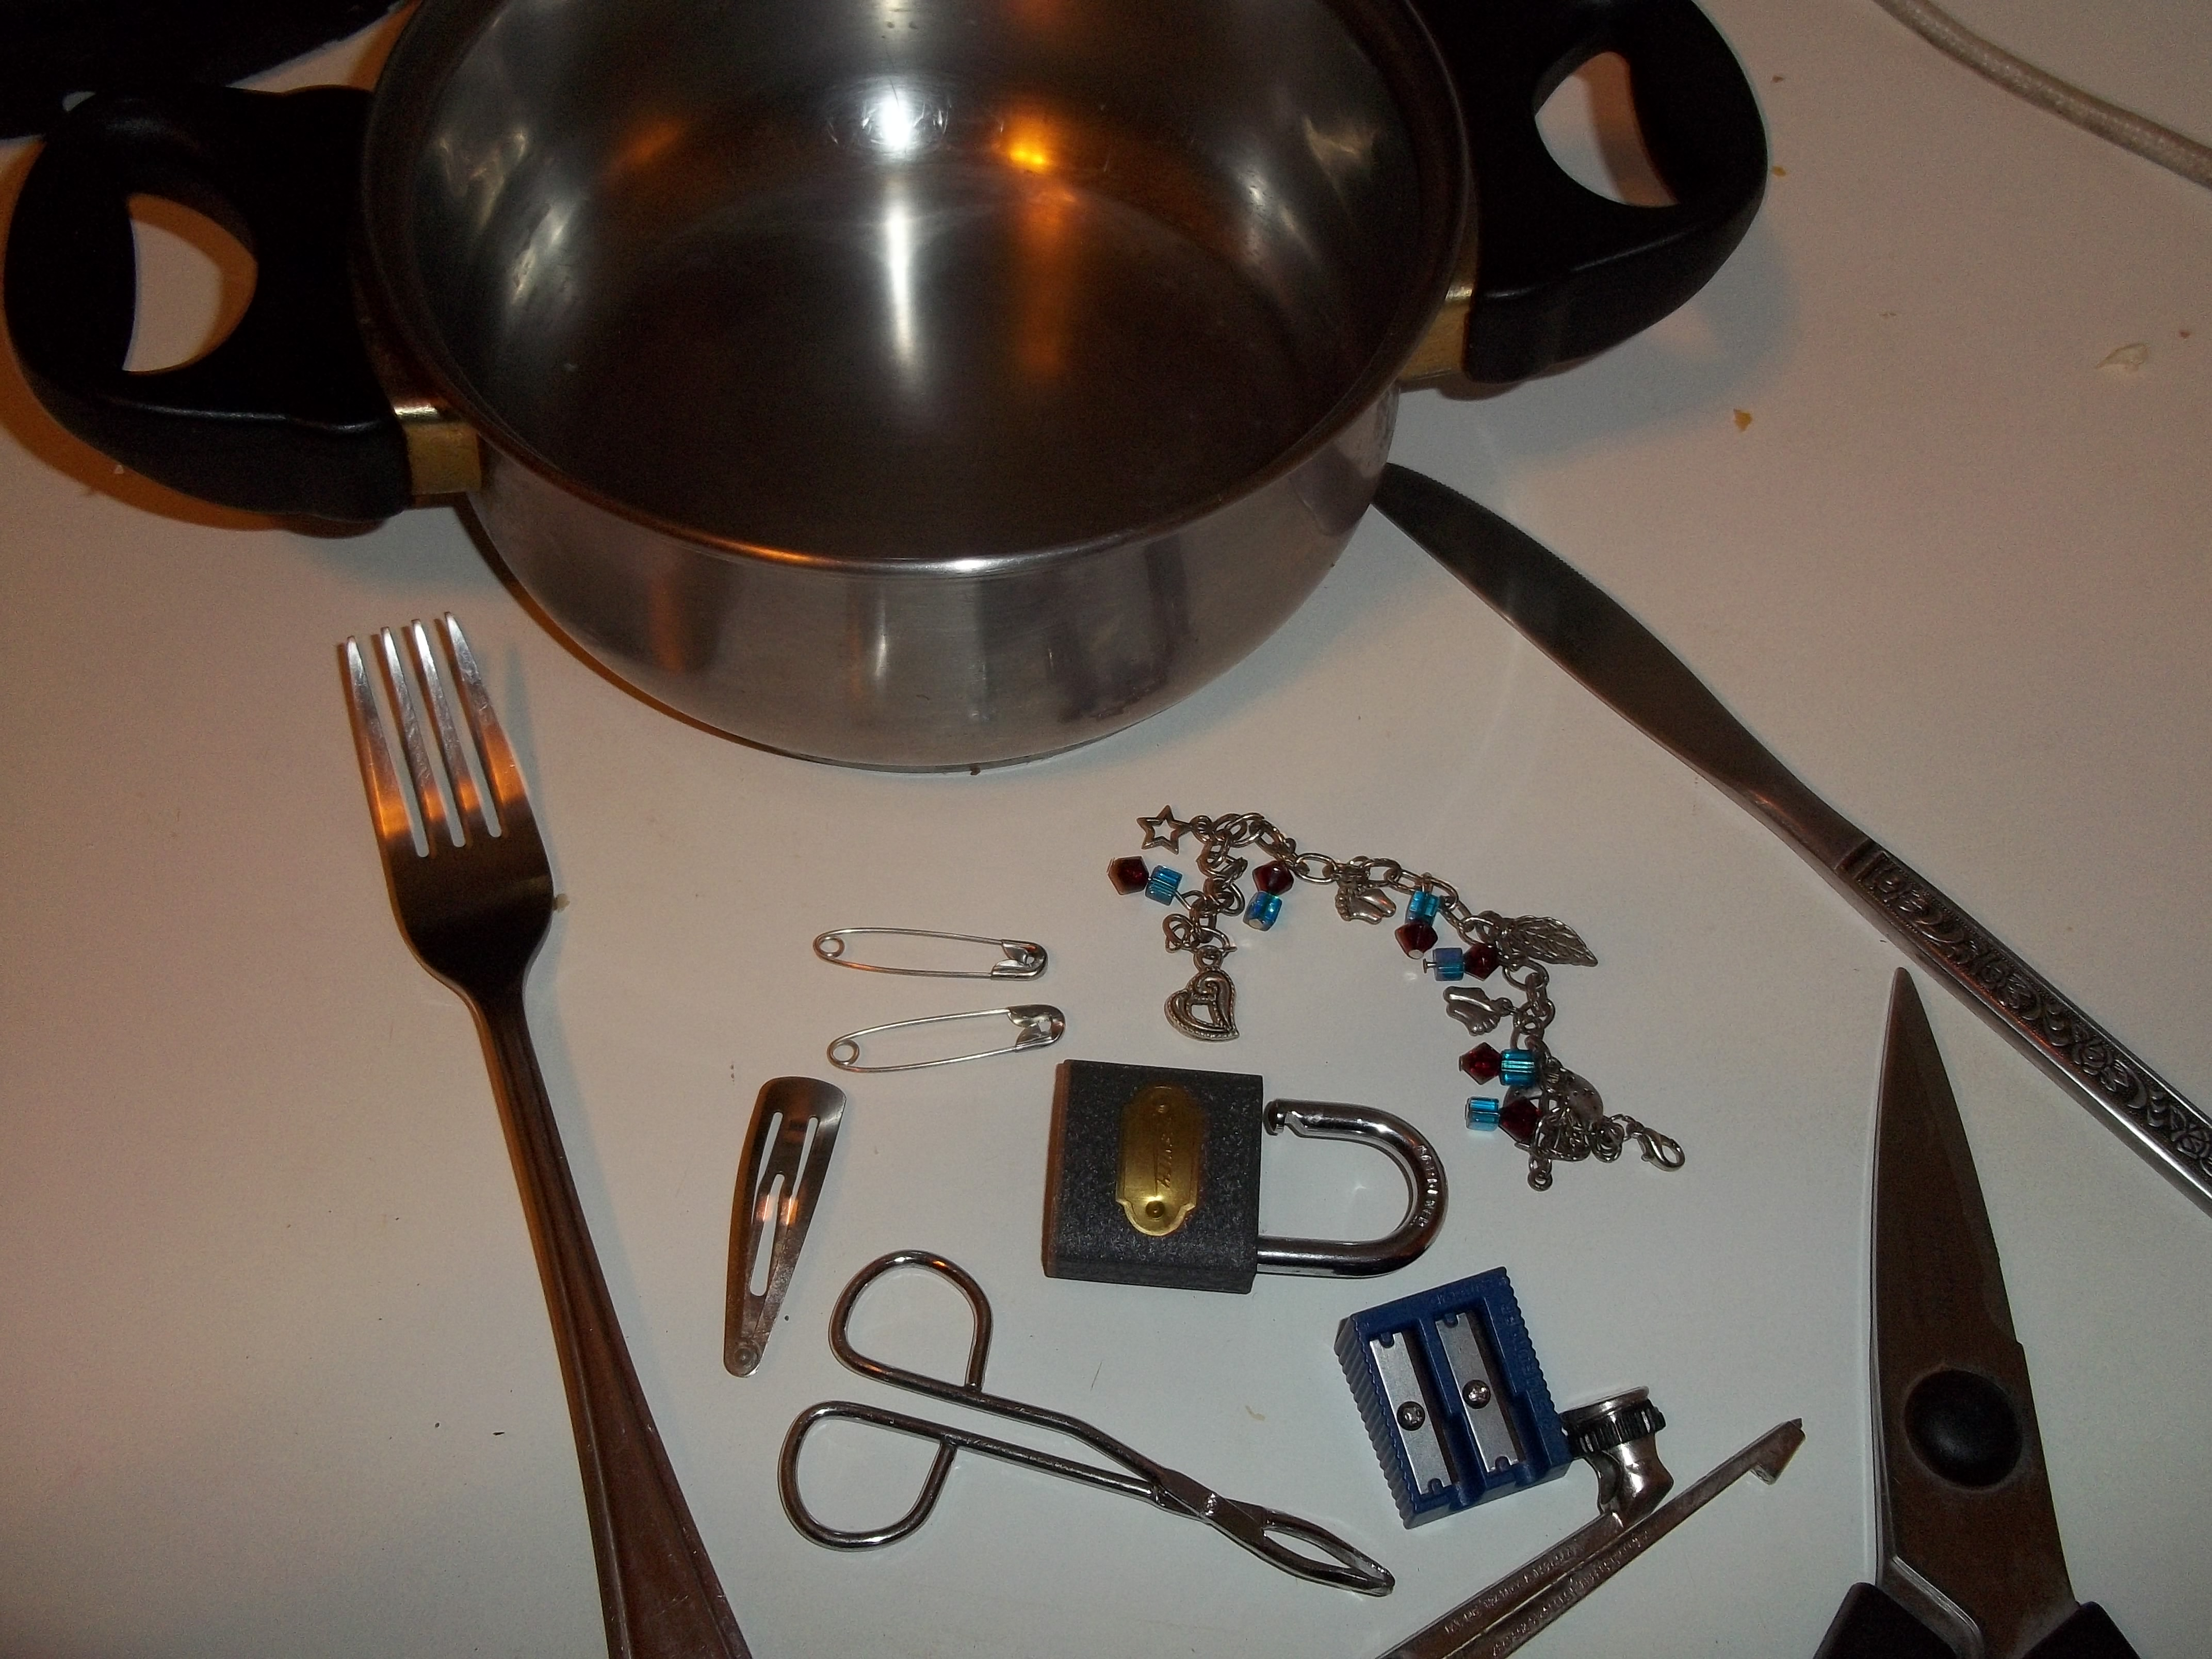
\includegraphics[width=.8\textwidth]{photos/metal_objects.jpg}\par
\end{center}
\end{minipage}
}
\end{activity}
      \label{m38708*uid93}
            \subsection*{Non-metals}
            \nopagebreak
\begin{minipage}{.5\textwidth}
        \label{m38708*id66021}In contrast to metals, non-metals are poor thermal conductors, good electrical insulators (meaning that they do \textsl{not} conduct electrical charge) and are neither malleable nor ductile. The non-metals include elements such as sulphur ($\text{S}$), phosphorus ($\text{P}$), nitrogen ($\text{N}$) and oxygen ($\text{O}$).\par 
\end{minipage}
\begin{minipage}{.5\textwidth}
\begin{center}
 \includegraphics[width=.4\textwidth]{photos/sulphurby-nickstone333.jpg}\par
\textit{Picture by nickstone333 on Flickr.com}
\end{center}
\end{minipage}
      \label{m38708*uid94}
            \subsection*{Metalloids}
            \nopagebreak
\begin{minipage}{.5\textwidth}
        \label{m38708*id66042}Metalloids or semi-metals have mostly non-metallic properties. One of their distinguishing characteristics is that their conductivity increases as their temperature increases. This is the opposite of what happens in metals. This property is known as semi-conductance and the materials are called semi-conductors. Semi-conductors are important in digital electronics, such as computers. The metalloids include elements such as silicon ($\text{Si}$) and germanium ($\text{Ge}$).\par 
\end{minipage}
\begin{minipage}{.5\textwidth}
\begin{center}
 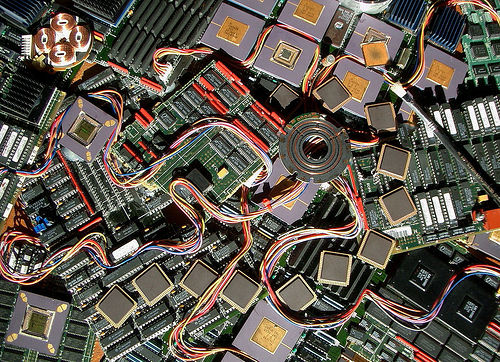
\includegraphics[width=.6\textwidth]{photos/siliconby-jurveston.jpg}\par
\textit{Picture by jurveston on Flickr.com}
\end{center}
\end{minipage}
\par \label{m38708*eip-586}\vspace{.5cm} 
      \noindent
   %   \hspace*{-30pt}
\includegraphics[width=0.5in]{col11305.imgs/pspencil2.png}   \raisebox{25mm}{   
   %   \begin{mdframed}[linewidth=4, leftmargin=40, rightmargin=40]  
%       \begin{wex}{Metals, metalloids and non-metals 1}{\label{m38708*eip-77}
%   \label{m38708*eip-252}
% For each of the following substances state whether they are metals, metalloids or non-metals, using their position on the periodic table.
% \label{m38708*eip-id1170734629720}
% \begin{enumerate}[noitemsep, label=\textbf{\alph*}. ] 
%             \leftskip=20pt\rightskip=\leftskip
% \item Oxygen
% \item Arsenic
% \item Vanadium
% \item Potassium
% \end{enumerate}
%   \par }
% {\vspace{5pt}
% %\label{m38708*eip-149}\noindent\textbf{Solution to Exercise }
% %\label{m38708*eip-id1170750216596}\begin{enumerate}[noitemsep, label=\textbf{\alph*}. ] 
% %            \leftskip=20pt\rightskip=\leftskip
% \westep {Look at the periodic table} 
% \begin{enumerate}[noitemsep, label=\textbf{\alph*}. ]
% \item Oxygen is on the right of the zigzag line and so is a non-metal.
% \item Arsenic is on the zigzag line and is a metalloid.
% \item Vanadium is on the left of zigzag line and so is a metal.
% \item Potassium is on the left of the zigzag line and so is a metal.\end{enumerate}
% }
%     \end{wex}
%  %   \end{mdframed}
%   %  }
% %    \noindent
%   \par
% %            \label{m38708*eip-173}\vspace{.5cm} 
% %      \noindent
% %      \hspace*{-30pt}
\includegraphics[width=0.5in]{col11305.imgs/pspencil2.png}   \raisebox{25mm}{   
% %      \begin{mdframed}[linewidth=4, leftmargin=40, rightmargin=40]  
%       \begin{wex}{Metals, metalloids and non-metals 2}{\label{m38708*eip-757}
%   \label{m38708*eip-25442}For each of the following substances state whether they are metals, metalloids or non-metals, using the information given.
% \label{m38708*eip-id1170742635239}
% \begin{enumerate}[noitemsep, label=\textbf{\alph*}. ] 
%             \leftskip=20pt\rightskip=\leftskip
% \item Aluminium in a cooking pot
% \item Silicon in a computer chip
% \item Plastic insulation around a wire
% \item Silver jewellery\end{enumerate}
%   \par }
% {\vspace{5pt}
% %\label{m38708*eip-1455}\noindent\textbf{Solution to Exercise }
% %\label{m38708*eip-id1170755988427}\begin{enumerate}[noitemsep, label=\textbf{\alph*}. ] 
%  %           \leftskip=20pt\rightskip=\leftskip
% \westep{Use what you know} \begin{enumerate}[noitemsep, label=\textbf{\alph*}. ]
% \item A cooking pot needs to be able to conduct heat and so the aluminium used must be a metal.
% \item Computer chips rely on semi-conductors and all metalloids are semiconductors. So silicon is a metalloid.
% \item The plastic around the wire must be insulating to current and so is a non-metal.
% \item Silver in the jewellery is chosen for its malleability and shiny lustre. So silver is a metal.
% \end{enumerate}}
%     \end{wex}
%    \end{mdframed}
%    }
    \noindent
%   \label{m38708**end}
%          \section{Properties}
%     \nopagebreak
    \label{m38706*cid6}
            \section{Electrical conductors, semi-conductors and insulators}
            \nopagebreak
            \label{m38706} $ \hspace{-5pt}\begin{array}{cccccccccccc}   
\includegraphics[width=0.75cm]{col11305.imgs/summary_simulation.png} &   
\includegraphics[width=0.75cm]{col11305.imgs/summary_video.png} &   \end{array} $ \hspace{2 pt}\raisebox{-5 pt}{} {(section shortcode: P10012 )} \par 
\label{m38706*id66058}An \textbf{electrical conductor} is a substance that allows an electrical current to pass through it. Electrical conductors are usually metals. \textsl{Copper} is one of the best electrical conductors, and this is why it is used to make conducting wire. In reality, \textsl{silver} actually has an even higher electrical conductivity than copper, but silver is too expensive to use. \par \\
\begin{minipage}{0.5\textwidth}
 In the overhead power lines that we see above us, \textsl{aluminium} is used. The aluminium usually surrounds a steel core which adds makes it stronger so that it doesn't break when it is stretched across distances. Sometimes gold is used to make wire because it is very resistant to surface corrosion. \textsl{Corrosion} is when a material starts to deteriorate because of its reactions with oxygen and water in the air.\par 
\end{minipage}
\begin{minipage}{.5\textwidth}
\begin{center}
 \includegraphics[height=.4\textwidth]{photos/Tripp.jpg}\par
\textit{Picture by Tripp on Flickr.com}
\end{center}
\end{minipage}
      \label{m38706*id66098}An \textbf{insulator} is a non-conducting material that does not carry any charge. Examples of insulators would be plastic and wood. \textbf{Semi-conductors} behave like insulators when they are cold, and like conductors when they are hot. The elements silicon and germanium are examples of semi-conductors.\par 
\Definition
%	  \begin{tabular*}{15 cm}{m{15 mm}m{}}
%	\hspace*{-50pt}  
\includegraphics[width=0.5in]{col11305.imgs/psflag2.png}   & \Definition{   \label{id2409398}\textbf{ 
{Conductors} 
%}} { \label{m38706*meaningfhsst!!!underscore!!!id354}
%      \label{m38706*id66124}
{A conductor allows the easy movement or flow of something such as heat or electrical charge through it.  \par 
       } 
\Definition{Insulators}
{Insulators are the opposite to conductors because they \textsl{inhibit} or reduce the flow of heat or electrical charge through them. \par}

%      \end{tabular*}
%      \end{definition}
\label{m38706*secfhsst!!!underscore!!!id357}
            \begin{g_experiment}{Electrical conductivity}{
            \nopagebreak
            \label{m38706*id66151}\noindent{}\textbf{Aim:}
        \newline
To investigate the electrical conductivity of a number of substances\par 
      \label{m38706*id66166}\noindent{}\textbf{Apparatus:} \\
\begin{minipage}{.5\textwidth}
      \label{m38706*id66175}\begin{itemize}[noitemsep]
            \label{m38706*uid95}\item two or three cells
\label{m38706*uid96}\item light bulb
\label{m38706*uid97}\item crocodile clips
\label{m38706*uid98}\item wire leads
\label{m38706*uid99}\item a selection of test substances (e.g. a piece of plastic, aluminium can, metal pencil sharpener, magnet, wood, chalk, cloth).
\end{itemize}
\end{minipage}
\begin{minipage}{.5\textwidth}
      \label{m38706*id66241}
    \setcounter{subfigure}{0}
	\begin{figure}[H] % horizontal\label{m38706*id66244}
    \begin{center}
\scalebox{0.7}{
\begin{pspicture}(0,-0.6)(5,6)
\SpecialCoor
%\psgrid[gridcolor=lightgray]
\pnode(0,0){A}
\pnode(0,5){B}
\pnode(5,5){C}
\pnode(5,0){D}
\pnode(3.5,0){E}
\pnode(1.5,0){F}
\rput{90}{\lamp(A)(B){light bulb}}
\battery(B)(C){cells}
\psline(C)(D)
\psline[arrowsize=10pt,arrowinset=0,arrowlength=2.5]{->}(D)(E)
\psframe(1.5,-0.5)(3.5,0.5)
\uput[u](2.5,0.5){test substance}
\rput(2.5,0){X}
\psline(4,0)(4,-0.4)(4.6,-0.4)
\uput[r](4.6,-0.4){crocodile clip}
\psline[arrowsize=10pt,arrowinset=0,arrowlength=2.5]{<-}(F)(A)
\end{pspicture}
}
    \end{center}
 \end{figure}  
\end{minipage}     
      \par 
      \label{m38706*id66251}\noindent{}\textbf{Method:}
        \newline
      \label{m38706*id66260}\begin{enumerate}[noitemsep, label=\textbf{\arabic*}. ] 
            \label{m38706*uid100}\item Set up the circuit as shown above, so that the test substance is held between the two crocodile clips. The wire leads should be connected to the cells and the light bulb should also be connected into the circuit.
\label{m38706*uid101}\item Place the test substances one by one between the crocodile clips and see what happens to the light bulb. If the light bulb shines it means that current is flowing and the substance you are testing is an \textbf{electrical conductor}.
\end{enumerate}
        \par 
      \label{m38706*id66291}\noindent{}\textbf{Results:}
        \newline
      Record your results in the table below:
    % \textbf{m38706*id66304}\par
          \begin{table}[H]
    % \begin{table}[H]
    % \\ '' '0'
        \begin{center}
      \label{m38706*id66304}
    \noindent
      \begin{tabular}{|p{2cm}|p{2cm}|p{2cm}|p{2cm}|}\hline
                \textbf{Test substance}
               &
                \textbf{Metal/non-metal}
               &
                \textbf{Does the light bulb glow?}
               &
                \textbf{Conductor or insulator}
            \\ \hline
         &
         &
         &
       \\ \hline
         &
         &
         &
       \\ \hline
         &
         &
         &
        \\ \hline
         &
         &
         &
        \\ \hline
    \end{tabular}
      \end{center}
\end{table}
    \par
  \par 
      \label{m38706*id66494}\noindent{}\textbf{Conclusions:}
        \newline
  In the substances that were tested, the metals were able to conduct electricity and the non-metals were not. Metals are good electrical conductors and non-metals are not.\par }
            \end{g_experiment}
\label{m38706*eip-316}The following simulation allows you to work through the above activity. For this simulation use the grab bag option to get materials to test. Set up the circuit as described in the activity.
    \setcounter{subfigure}{0}
	\begin{figure}[H] % horizontal\label{m38806*transverse-waves}
    \textnormal{Phet simulation for electrical conductivity}\vspace{.1in} \nopagebreak
  \label{m38806*phet!!!underscore!!!sim}\label{m38806*phet-simulation}
            \raisebox{-5 pt}{ 
\includegraphics[width=0.5cm]{col11305.imgs/summary_www.png}} { (Simulation:  lbK )}
      \vspace{2pt}
    \vspace{.1in}
 \end{figure}    
        \par 
    \label{m38706*cid7}
            \section{Thermal Conductors and Insulators}
            \nopagebreak
      \label{m38706*id66527}A \textbf{thermal conductor} is a material that allows energy in the form of heat, to be transferred within the material, without any movement of the material itself. An easy way to understand this concept is through a simple demonstration.\par 
\label{m38706*secfhsst!!!underscore!!!id453}
            \begin{g_experiment}{Demonstration: Thermal conductivity}{
            \nopagebreak
            \label{m38706*id66568}\noindent{}\textbf{Aim: }\newline
    To demonstrate the ability of different substances to conduct heat.\par 
      \label{m38706*id66588}\noindent{}\textbf{Apparatus: }\newline
\begin{minipage}{.5\textwidth}
You will need:
\begin{itemize}
 \item two cups (made from the same material e.g. plastic)
\item a metal spoon
\item a plastic spoon.
\end{itemize} 
\end{minipage}
\begin{minipage}{.5\textwidth}
	\begin{figure}[H] % horizontal\label{m38706*id66244}
    \begin{center}
\scalebox{0.5}{
\begin{pspicture}(-5,-5)(5,5)
\psset{unit=1cm}
\newpsstyle{white} {linestyle=solid,linewidth=.1,fillstyle=none}
\uput[r](-3,1){\Large{boiling water}}
\psline[linewidth=0.04]{->}(-0.3,1)(0.5,1)
\uput[r](-3,3){\Large{plastic spoon}}
\psline[linewidth=0.04]{->}(-0.25,3)(0.2,3)
\psline[linewidth=0.1](1.95,0)(0.25,3.2)
\pstTubeEssais[glassType=becher,aspectLiquide1=white]
\uput[r](3.5,1){\Large{boiling water}}
\psline[linewidth=0.04]{->}(3.55,1)(2.6,1)
\uput[r](3.5,3){\Large{metal spoon}}
\psline[linewidth=0.04]{->}(3.55,3)(3,3)
\psline[linewidth=0.1](0.95,0)(3,3.2)
\pstTubeEssais[glassType=becher,aspectLiquide1=white]
\end{pspicture}}
    \end{center}
 \end{figure} 
\end{minipage}
      \label{m38706*id66592}\textbf{Method:}
\label{m38706*id66609}\begin{itemize}[noitemsep]
\label{m38706*uid102}\item Pour boiling water into the two cups so that they are about half full.
\label{m38706*uid103}\item Place a metal spoon into one cup and a plastic spoon in the other.
\label{m38706*uid104}\item Note which spoon heats up more quickly
\end{itemize}
        \par 
\label{m38706*eip-270}
%\begin{tabular}{cc}
%	\hspace*{-50pt}\raisebox{-8 mm}{\hspace{-0.2in}
\includegraphics[width=0.5in]{col11305.imgs/pstip2.png} } & 
%	\begin{minipage}{0.85\textwidth}
%	\begin{note}
      \Warning{Be careful when working with boiling water and when you touch the spoons as you can easily burn yourself.}
%	\end{note}
%	\end{minipage}
%	\end{tabular}
	\par
      \label{m38706*id66666}\noindent{}\textbf{Results: }\newline
    The metal spoon heats up faster than the plastic spoon. In other words, the metal conducts heat well, but the plastic does not.\par 
\label{m38706*id66687}\noindent{}\textbf{Conclusion: }Metal is a good thermal conductor, while plastic is a poor thermal conductor.}
\end{g_experiment}
 \par 
      \label{m38706*id66699}An \textbf{insulator} is a material that does not allow a transfer of electricity or energy. Materials that are poor thermal conductors can also be described as being good thermal insulators.\par 
% \label{m38706*notfhsst!!!underscore!!!id490}
% \begin{tabular}{cc}
% 	\hspace*{-50pt}\raisebox{-8 mm}{\hspace{-0.2in}
\includegraphics[width=0.75in]{col11305.imgs/psfact2.png} } & 
% 	\begin{minipage}{0.85\textwidth}
% 	\begin{note}
%       {note: }Water is a better thermal conductor than air and conducts heat away from the body about 20 times more efficiently than air. A person who is not wearing a wetsuit, will lose heat very quickly to the water around them and can be vulnerable to hypothermia (this is when the body temperature drops very low). Wetsuits help to preserve body heat by trapping a layer of water against the skin. This water is then warmed by body heat and acts as an insulator. Wetsuits are made out of closed-cell, foam neoprene. Neoprene is a synthetic rubber that contains small bubbles of nitrogen gas when made for use as wetsuit material. Nitrogen gas has very low thermal conductivity, so it does not allow heat from the body (or the water trapped between the body and the wetsuit) to be lost to the water outside of the wetsuit. In this way a person in a wetsuit is able to keep their body temperature much higher than they would otherwise.
% 	\end{note}
% 	\end{minipage}
% 	\end{tabular}
	\par
\label{m38706*secfhsst!!!underscore!!!id492}
            \begin{Investigation}{A closer look at thermal conductivity}
{            \nopagebreak
      \label{m38706*id66744}Look at the table below, which shows the thermal conductivity of a number of different materials, and then answer the questions that follow. The higher the number in the second column, the better the material is at conducting heat (i.e. it is a good thermal conductor). Remember that a material that conducts heat efficiently, will also lose heat more quickly than an insulating material.\par 
    % \textbf{m38706*id66753}\par
          \begin{table}[H]
    % \begin{table}[H]
    % \\ '' '0'
        \begin{center}
      \label{m38706*id66753}
    \noindent
      \begin{tabular}{|l|l|}\hline
\textbf{Material} & \textbf{Thermal Conductivity} \\ 
                 &  \textbf{($\text{W}\ensuremath{\cdot}\text{m}{}^{-1}\ensuremath{\cdot}\text{K}{}^{-1}$) } \\ \hline
Silver & 429 \\ \hline
Stainless steel & 16 \\ \hline
Standard glass & 1.05 \\ \hline
Concrete & 0.9 - 2 \\ \hline
Red brick & 0.69 \\ \hline
Water & 0.58 \\ \hline
Polyethylene (plastic) & 0.42 - 0.51 \\ \hline
Wood & 0.04 - 0.12 \\ \hline
Polystyrene & 0.03 \\ \hline
Air & 0.024 \\ \hline
    \end{tabular}
      \end{center}
%    \begin{center}{\small\bfseries Table 1.4}\end{center}
%    \begin{caption}{\small\bfseries Table 1.4}\end{caption}
\end{table}
    \par
      \label{m38706*id67009}Use this information to answer the following questions:\par 
      \label{m38706*id67013}\begin{enumerate}[noitemsep, label=\textbf{\arabic*}. ] 
            \label{m38706*uid105}\item Name two materials that are good thermal conductors.
\label{m38706*uid106}\item Name two materials that are good insulators.
\label{m38706*uid107}\item Explain why:
\label{m38706*id67053}\begin{enumerate}[noitemsep, label=\textbf{\alph*}. ] 
            \label{m38706*uid108}\item Red brick is a better choice than concrete for building houses that need less internal heating. 
\label{m38706*uid109}\item Stainless steel is good for making cooking pots
\end{enumerate}
        \end{enumerate}}
\end{Investigation}
\label{m38706*notfhsst!!!underscore!!!id564}
%\begin{tabular}{cc}
%	\hspace*{-50pt}\raisebox{-8 mm}{\hspace{-0.2in}
\includegraphics[width=0.75in]{col11305.imgs/psfact2.png} } & 
%	\begin{minipage}{0.85\textwidth}
%	\begin{note}
      \IFact{Well-insulated buildings need less energy for heating than buildings that have no insulation. Two building materials that are being used more and more worldwide, are \textbf{mineral wool} and \textbf{polystyrene}. Mineral wool is a good insulator because it holds air still in the matrix of the wool so that heat is not lost. Since air is a poor conductor and a good insulator, this helps to keep energy within the building. Polystyrene is also a good insulator and is able to keep cool things cool and hot things hot. It has the added advantage of being resistant to moisture, mould and mildew.}
%	\end{note}
%	\end{minipage}
%	\end{tabular}
	\par
    \label{m38706*cid8}
            \section{Magnetic and Non-magnetic Materials}
            \nopagebreak
      \label{m38706*id67151}We have now looked at a number of ways in which matter can be grouped, such as into metals, semi-metals and non-metals; electrical conductors and insulators, and thermal conductors and insulators. One way in which we can further group metals, is to divide them into those that are \textbf{magnetic} and those that are \textbf{non-magnetic.}\par 
\par
%             \label{m38706*fhsst!!!underscore!!!id570}\begin{definition}
% 	  \begin{tabular*}{15 cm}{m{15 mm}m{}}
% 	\hspace*{-50pt}  
\includegraphics[width=0.5in]{col11305.imgs/psflag2.png}   & 
\Definition{   \label{id2410309} { Magnetism }} { \label{m38706*meaningfhsst!!!underscore!!!id570}
      \label{m38706*id67174}Magnetism is a force that certain kinds of objects, which are called `magnetic' objects, can exert on each other without physically touching. A magnetic object is surrounded by a magnetic `field' that gets weaker as one moves further away from the object. \par 
       } 
%       \end{tabular*}
%       \end{definition}
\begin{minipage}{.5\textwidth}
      \label{m38706*id67186}A metal is said to be \textbf{ferromagnetic} if it can be magnetised (i.e. made into a magnet). If you hold a magnet very close to a metal object, it may happen that its own electrical field will be induced and the object becomes magnetic. Some metals keep their magnetism for longer than others. Look at iron and steel for example. Iron loses its magnetism quite quickly if it is taken away from the magnet. Steel on the other hand will stay magnetic for a longer time. Steel is often used to make permanent magnets that can be used for a variety of purposes.\par 
\end{minipage}
\begin{minipage}{.5\textwidth}
\begin{center}
 \includegraphics[width=.8\textwidth]{photos/magnet.jpg}\par
\textit{Picture by Aney on wikimedia}
\end{center}
\end{minipage}
      \label{m38706*id67200}Magnets are used to sort the metals in a scrap yard, in compasses to find direction, in the magnetic strips of video tapes and ATM cards where information must be stored, in computers and TV's, as well as in generators and electric motors.\par 
\label{m38706*secfhsst!!!underscore!!!id575}
            \begin{Investigation}{Magnetism}{
            \nopagebreak
      \label{m38706*id67220}You can test whether an object is magnetic or not by holding another magnet close to it. If the object is attracted to the magnet, then it too is magnetic.\par 
      \label{m38706*id67227}Find five objects in your classroom or your home and test whether they are magnetic or not. Then complete the table below:\par 
    % \textbf{m38706*id67234}\par
          \begin{table}[H]
    % \begin{table}[H]
    % \\ '' '0'
        \begin{center}
      \label{m38706*id67234}
    \noindent
      \begin{tabular}{|l|l|}\hline
                \textbf{Object}
               &
                \textbf{Magnetic or non-magnetic} \\ \hline
         & \\ \hline
         & \\ \hline
         & \\ \hline
         & \\ \hline
         & \\ \hline
    \end{tabular}
      \end{center}
%     \begin{center}{\small\bfseries Table 1.5}\end{center}
%     \begin{caption}{\small\bfseries Table 1.5}\end{caption}
\end{table}}

\end{Investigation}
    \par
\label{m38706*secfhsst!!!underscore!!!id616}
            \begin{groupdiscussion}{Group Discussion : Properties of materials}{
            \nopagebreak
      \label{m38706*id67392}In groups of 4-5, discuss how knowledge of the properties of materials has allowed::\par 
      \label{m38706*id67398}\begin{itemize}[noitemsep]
            \label{m38706*uid111}\item society to develop advanced computer technology
\label{m38706*uid112}\item homes to be provided with electricity
\label{m38706*uid113}\item society to find ways to conserve energy
\item indigenous peoples to cook their food
\end{itemize}
\end{groupdiscussion}
\label{m38706*eip-968}The following presentation provides a summary of the classification of matter.
    \setcounter{subfigure}{0}
	\begin{figure}[H] % horizontal\label{m38706*slidesharefigure}
    \label{m38706*slidesharemedia}\label{m38706*slideshareflash}\raisebox{-5 pt}{ 
\includegraphics[width=0.5cm]{col11305.imgs/summary_www.png}} { (Presentation:  P10013 )}
      \vspace{2pt}
    \vspace{.1in}
 \end{figure}       \par}
\end{discussion} \label{m38706*cid9}
            \section{Summary}
            \nopagebreak
      \label{m38706*id67458}\begin{itemize}[noitemsep]
            \label{m38706*uid114}\item All the objects and substances that we see in the world are made of \textbf{matter}.
\label{m38706*uid115}\item This matter can be classified according to whether it is a \textbf{mixture} or a \textbf{pure substance}.
\label{m38706*uid116}\item A \textbf{mixture} is a combination of one or more substances that are not chemically bonded to each other. Examples of mixtures are air (a mixture of different gases) and cereal in milk.
\label{m38706*uid117}\item The main \textbf{characteristics} of mixtures are that the substances that make them up are not in a fixed ratio, they keep their individual properties and they can be separated from each other using mechanical means.
\label{m38706*uid118}\item A \textbf{heterogeneous mixture} is non-uniform and the different parts of the mixture can be seen. An example would be a mixture of sand and water.
\label{m38706*uid119}\item A \textbf{homogeneous mixture} is uniform, and the different components of the mixture can't be seen. An example would be salt in water.
\label{m38706*uid121}\item Pure substances can be further divided into \textbf{elements} and \textbf{compounds}.
\label{m38706*uid122}\item An \textbf{element} is a substance that can't be broken down into simpler substances through chemical means.
\label{m38706*uid123}\item All the elements are recorded in the \textbf{periodic table}. Each element has its own chemical symbol. Examples are iron ($\text{Fe}$), sulphur ($\text{S}$), calcium ($\text{Ca}$), magnesium ($\text{Mg}$) and fluorine ($\text{F}$).
\label{m38706*uid124}\item A \textbf{compound} is a substance that is made up of two or more elements that are chemically bonded to each other in a fixed ratio. Examples of compounds are sodium chloride ($\text{NaCl}$), iron sulphide ($\text{FeS}$), calcium carbonate (${\text{CaCO}}_{3}$) and water (${\text{H}}_{2}\text{O}$).
\label{m38706*uid125}\item When \textbf{naming compounds} and writing their \textbf{chemical formula}, it is important to know the elements that are in the compound, how many atoms of each of these elements will combine in the compound and where the elements are in the periodic table. A number of rules can then be followed to name the compound.
\label{m38706*uid126}\item Another way of classifying matter is into \textbf{metals} (e.g. iron, gold, copper), \textbf{metalloids} (e.g. silicon and germanium) and \textbf{non-metals} (e.g. sulphur, phosphorus and nitrogen).
\label{m38706*uid127}\item \textbf{Metals} are good electrical and thermal conductors, they have a shiny lustre, they are malleable and ductile, and they have a high melting point. These properties make metals very useful in electrical wires, cooking utensils, jewellery and many other applications.
\label{m38706*uid128}\item A further way of classifying matter is into \textbf{electrical conductors}, \textbf{semi-conductors} and \textbf{insulators}.
\label{m38706*uid129}\item An \textbf{electrical conductor} allows an electrical current to pass through it. Most metals are good electrical conductors.
\label{m38706*uid130}\item An \textbf{electrical insulator} is not able to carry an electrical current. Examples are plastic, wood, cotton material and ceramic.
\label{m38706*uid131}\item Materials may also be classified as \textbf{thermal conductors} or \textbf{thermal insulators} depending on whether or not they are able to conduct heat.
\label{m38706*uid132}\item Materials may also be \textbf{magnetic} or \textbf{non-magnetic}.
\end{itemize} \pagebreak

\label{m38706*secfhsst!!!underscore!!!id672}
            \begin{eocexercises}{Classification of matter }{
            \nopagebreak
      \label{m38706*id67920}\begin{enumerate}[noitemsep, label=\textbf{\arabic*}. ] 
            \label{m38706*uid133}\item For each of the following \textbf{multiple choice} questions, choose \textsl{one} correct answer from the list provided.
\label{m38706*id67947}\begin{enumerate}[noitemsep, label=\textbf{\alph*}. ] 
            \label{m38706*uid134}\item Which of the following can be classified as a mixture:
\label{m38706*id67963}\begin{enumerate}[noitemsep, label=\textbf{\roman*}. ] 
            \label{m38706*uid135}\item sugar
\label{m38706*uid136}\item table salt
\label{m38706*uid137}\item air
\label{m38706*uid138}\item iron
\end{enumerate}
                \label{m38706*uid139}\item An element can be defined as:
\label{m38706*id68029}\begin{enumerate}[noitemsep, label=\textbf{\roman*}.] 
            \label{m38706*uid140}\item A substance that cannot be separated into two or more substances by ordinary chemical (or physical) means
\label{m38706*uid141}\item A substance with constant composition
\label{m38706*uid142}\item A substance that contains two or more substances, in definite proportion by weight
\label{m38706*uid143}\item A uniform substance
\end{enumerate}
                \end{enumerate}
\label{m38706*uid144}\item Classify each of the following substances as an \textsl{element}, a \textsl{compound}, a \textsl{homogeneous mixture}, or a \textsl{heterogeneous mixture}: salt, pure water, soil, salt water, pure air, carbon dioxide, gold and bronze.\newline
\label{m38706*uid145}\item Look at the table below. In the first column (A) is a list of substances. In the second column (B) is a description of the group that each of these substances belongs in. Match up the \textsl{substance} in Column A with the \textsl{description} in Column B.
    % \textbf{m38706*id68147}\par
          \begin{table}[H]
    % \begin{table}[H]
    % \\ 'id2880342' '1'
        \begin{center}
      \label{m38706*id68147}
      \begin{tabular}{|l|l|}\hline
\textbf{Column A} & \textbf{Column B} \\ \hline
iron & a compound containing 2 elements \\ \hline
H$_\text{2}$S & a heterogeneous mixture \\ \hline
sugar solution & a metal alloy \\ \hline
sand and stones & an element \\ \hline
steel & a homogeneous mixture \\ \hline
    \end{tabular}
      \end{center}
%     \begin{center}{\small\bfseries Table 1.6}\end{center}
%     \begin{caption}{\small\bfseries Table 1.6}\end{caption}
\end{table}
    \par
\label{m38706*uid146}\item You are given a test tube that contains a mixture of iron filings and sulphur. You are asked to weigh the amount of iron in the sample.
\label{m38706*id68262}\begin{enumerate}[noitemsep, label=\textbf{\alph*}. ] 
            \label{m38706*uid147}\item Suggest one method that you could use to separate the iron filings from the sulphur.
\label{m38706*uid148}\item What property of metals allows you to do this?
\end{enumerate}
\label{m38706*uid149}\item Given the following descriptions, write the chemical formula for each of the following substances:
\label{m38706*id68304}\begin{enumerate}[noitemsep, label=\textbf{\alph*}. ] 
            \label{m38706*uid150}\item silver metal
\label{m38706*uid151}\item a compound that contains only potassium and bromine
\label{m38706*uid152}\item a gas that contains the elements carbon and oxygen in a ratio of 1:2
\end{enumerate}
\label{m38706*uid153}\item Give the names of each of the following compounds:
\label{m38706*id68358}\begin{enumerate}[noitemsep, label=\textbf{\alph*}. ] 
            \label{m38706*uid154}\item $\text{NaBr}$
\label{m38706*uid155}\item ${\text{Ba}(\text{NO}}}_{2})_2$
\label{m38706*uid156}\item ${\text{SO}}_{2}$ 
\item $\text{H}_{2}\text{SO}_{4}$
\end{enumerate}
\item Give the formula for each of teh following compounds:
\begin{enumerate}[noitemsep, label=\textbf{\alph*}.]
 \item iron (II) sulphate
\item boron trifluoride
\item potassium permanganate
\item zinc chloride
\end{enumerate}

\label{m38706*uid157}\item For each of the following materials, say what properties of the material make it important in carrying out its particular function.
\label{m38706*id68436}\begin{enumerate}[noitemsep, label=\textbf{\alph*}. ] 
            \label{m38706*uid158}\item \textbf{tar} on roads
\label{m38706*uid159}\item \textbf{iron} burglar bars
\label{m38706*uid160}\item \textbf{plastic} furniture
\label{m38706*uid161}\item \textbf{metal} jewellery
\label{m38706*uid162}\item \textbf{clay} for building
\label{m38706*uid163}\item \textbf{cotton} clothing
\end{enumerate}
\end{enumerate}
  \label{m38706**end}
  \label{09a7a4809656be0b739ee130746cd803**end}
\par \raisebox{-5 pt}{
\includegraphics[width=0.5cm]{col11305.imgs/summary_www.png}} Find the answers with the shortcodes:
 \par \begin{tabular}[h]{cccccc}
 (1.) ll6  &  (2.) llF  &  (3.) llG  &  (4.) ll7  &  (5.) llA  &  (6.) llo  &  (7.) lls  &  (8.) llH  & \end{tabular}}
\end{eocexercises}
